\documentclass[a4paper]{article}

\usepackage[backend=biber,natbib=true,style=authoryear-comp,doi=false,url=false,isbn=false]{biblatex}
\bibliography{paper}

\usepackage[utf8]{inputenc}
\usepackage{todonotes}
\usepackage{a4wide}
\usepackage{amsmath}
\usepackage{amssymb}
\usepackage{syllogism}
\usepackage{subcaption}
\usepackage{rotating}


\usepackage{xcolor}
\definecolor{Red}{RGB}{178,34,34}
\newcommand{\mf}[1]{\textcolor{Red}{[mf: #1]}}

\begin{document}

\title{Towards an ecology of vagueness}
\author{Jos\'e Pedro Correia \and Michael Franke}
\date{}

\maketitle

\begin{abstract}
A vexing puzzle about vagueness, rationality and evolution runs, in crude abbreviation, as follows: vague language use is demonstrably suboptimal if the goal is efficient precise and cooperative information transmission; hence rational deliberation or evolutionary selection should, under this assumed goal, eradicate vagueness from language use.
Since vagueness is persistent in all human languages, something has to give.
In this paper, we focus on this problem in the context of signaling games.
We provide an overview of a number of proposed reasons why and mechanisms how vagueness may come into the picture in formal models of rational or evolutionary signaling.
Most of them argue that vague signal use is simply the best we can get, given certain factors.
Despite the plausibility of the proposals, we argue that a deeper understanding of the benefits of vagueness needs a more ecological perspective, namely one that goes beyond local optimization of signaling strategies of a homogeneous population.
As an example of one possible way to expand upon our current models, we propose two variants of a novel multi-population dynamic of imprecise imitation where, under certain conditions, populations with a certain level of imprecision dominate over precise ones.
\end{abstract}

\tableofcontents


\section{Vagueness and the classical picture}
\label{sec:vagueness}

The classical philosophical problem of vagueness is most starkly embodied by the sorites paradox.
The original formulation is attributed to Eubulides, an ancient Megarian philosopher~\parencite{sorensen_sorites_2009}, and uses the example of a heap of sand: if no removal of one grain of sand can make a heap into a non-heap, we can repeatedly remove all but one grain of sand of something that is clearly a heap and be forced to acknowledge that the remaining single grain of sand is still a heap; otherwise, it seems, we would have to accept that there is a determinate number of grains that forms a heap, and anything under it is not a heap.
Neither choice is, however, intuitively satisfying.
The paradox is interesting because it can be made general and re-applied to many other words besides `heap'.
Predicates for which one can find a suitable instance of the general formulation of the sorites paradox are called \emph{vague}.
Paradigmatic examples besides `heap' include `tall', `red', `bald', `tadpole', and `child'~\parencite{Keefe1997}.
How widespread is the problem?
It is easy to find more examples of predicates based on more finely grained properties---as `tall' is intuitively based on height---for which constructing a sorites paradox would be easy.
Mereological nihilists argue that instances of the sorites can be designed for any material object that can be decomposed into small enough parts.
If we subscribe to the scientific picture of matter as composed of molecules and atoms, this applies to tables and chairs, cats and mats, and any other ordinary thing~\parencite{Unger1979}.
Bertrand Russell famously argued~\parencite*{russell_vagueness_1923} that all words, including ``the words of pure logic'', are vague when used by human beings.
If we think of language as governed by logical rules, and of rationality as the ability to follow those rules, the sorites paradox seems \emph{prima facie} to show that vagueness in our language can undermine our rationality.

But we can think of language in different terms.
A possibility is to think of signs as tools agents use to coordinate actions.
An example of a way to formally study language along those lines is by using the framework of signaling games~\parencite{lewis_convention_1969}.
In such a context, rationality becomes the ability to choose the use of signs that is optimal to achieve the desired coordination.
%So what about vagueness?
However, in the context of these game-theoretic approaches to language, vagueness presents a new challenge.
Barton Lipman~\parencite*{lipman_why_2009} gives a detailed account of the problem.
Very succinctly, it can be put as follows.
In standard game-theoretic models of communication, vague signal use yields a lower expected utility than crisp use.
Therefore, given that the dynamics (be it natural selection, cultural evolution, or rational choice) maximize utility, vagueness should be weeded out by these forces, giving rise to only precise languages.
Thus it would be irrational to stick to vague language use when we could (theoretically) switch to a better system.
But as we said before, vagueness is pervasive in our natural languages, and there is no reason to believe it is going away.
The problem seems to be a theoretically serious one, but it does not obviously undermine our everyday linguistic practices.
Most of the time we seem to communicate just fine.
Therefore, the issue must lie with the conceptions we have of the forces or mechanisms that underlie those practices.
Lipman concludes that ``we cannot explain the prevalence of vague terms in natural language without a model of bounded rationality which is significantly different from anything in the existing literature''~\parencite*[1]{lipman_why_2009}.

%Vagueness is typically seen as a challenge to a classical conception of language that relies on reference and truth as two core notions for understanding meaning.
%One problem is that vague predicates seem to lack precise boundaries; if that is the case, how can words like `tall' stand in correspondence to something like a well defined set of tall people?
%And if we cannot know exactly whether a certain person is `tall' or not, as with borderline cases, how are we to determine the truth value of sentences that involve statements of tallness regarding these borderline cases?
%Supervaluationism, many-valued logics, and degree theories all propose changes to the classical picture in order to accommodate for vague predicates.
%They are, however, still strongly committed to its two core notions.
%As argued by Mark Sainsbury~\parencite*{sainsbury_concepts_1999}, because of that they fail to address an important characteristic of vague predicates: \emph{higher order vagueness}.
%All the aforementioned proposals end up being committed to new artificial demarcating boundaries (\emph{e.g.}~true-under-all-precisifications versus neither true nor false versus false-under-all-precisifications, true versus indefinite versus false, true to degree 1 versus true to degree 0 versus the rest).
%But a vague predicate not only fails to demarcate between the cases where it clearly applies and the ones where it clearly doesn't, it also fails to establish a boundary between the cases where it clearly applies and the borderline cases, as well as between the borderline cases and the cases where it clearly doesn't apply.
%Further introducing borderline borderline cases would lead to an infinite regress.
%Because of their attachment to the classical picture, the standard approaches to vagueness also fail to draw an important lesson from the sorites paradox, namely that ``we do not know, cannot know, and do not need to know these supposed boundaries to use language correctly''~\parencite*[256]{sainsbury_concepts_1999}.
% \begin{quote}
% But to what in our actual use of language does this division correspond?
% It looks as if, as before, it should correspond to the sentences true beyond the shadow of vagueness, those in some kind of borderline position, and those false beyond the shadow.
% But [\ldots] we do not know, cannot know, and do not need to know these supposed boundaries to use language correctly.
% Hence they cannot be included in a correct description of our language.%
% ~\parencite[256]{sainsbury_concepts_1999}
% \end{quote}
%By trying to cling as much as possible to the classical picture of logic and semantics, these standard approaches are ignoring a simple observation: natural language users are sensitive to the sorites paradox, \emph{i.e.}~they are able to recognize the logical inconsistency but do not have a good answer as to how to overcome it.
%Even more importantly, they apparently do not need to solve the inconsistency in order to continue using natural language to achieve their daily goals.
%Nobody ever stopped using the word `tall` after being confronted with a sorites series.
%Why should we develop theories of meaning that are impervious to the paradox?
%
%The reluctance to give up truth and logic as valuable notions to explain meaning is perhaps associated with the fear of what would also need to be abandoned as a consequence.
%One notion that seems to quickly be in peril is that of rationality.
%In reference to philosophers who defend the desirability of a classical notion of truth, Richard Rorty says:
%\begin{quote}
%In the past, such philosophers have typically conjoined the claim that there is universal human agreement on the supreme desirability of truth with two further premises: that truth is correspondence to reality, and that reality has an intrinsic nature (that there is, in Nelson Goodman's terms, a Way the World Is).
%[\ldots]
%The rise of relatively democratic, relatively tolerant, societies in the last few hundred years is said to be due to the increased rationality of modern times, where `rationality' denotes the employment of an innate truth-oriented faculty.%
%~\parencite*[1]{rorty_response_2000-1}
%\end{quote}
%By tying all of these notions tightly together, the fear could be that by dropping the picture of meaning as intimately tied to truth and logic we necessarily lose the ground on which rationality stands, and the whole edifice could collapse.
%Rationality, in this picture, has truth as its guiding light and logic as the means to attain it.
%Being rational is about following universally valid rules of reasoning that, given the correct inputs, necessarily lead us to the correct conclusions. % (see, for example, Harold Brown~\parencite*[19]{brown_rationality_1990} for a characterization).
%Although humans are not necessarily consciously aware of the rules, they are considered to be nevertheless unconsciously following them when they act rationally.
%This type of rationality is one that supposedly demarcates humans from other animals.

%We want to argue here that to say that language does not follow strict logical rules, or that truth is not a useful notion to guide our inquiries into meaning, is not to say that language is unstructured, meaningless, or unusable; neither is it to say that we, language users, are therefore irrational.
%Giving up the ideal of truth and logic as relevant explanatory notions for understanding meaning in natural language does not imply giving up on rationality altogether.
%It also does not necessarily eradicate all hope for a (formal) explication of meaning.
%In order to make this argument, we need a different paradigm of language and meaning.
%But what could such a paradigm even be?
%
%We suggest that inspiration can be drawn from the later work of philosopher Ludwig Wittgenstein%
%\footnote{To the extent that substantial views can be said to be defended by the author. Skipping over the debate (but see~\cite{kahane_wittgenstein_2007} for more details), we are here assuming an interpretation of Wittgenstein as a kind of pragmatist, along the lines of the readings of Hilary Putnam~\parencite*{putnam_pragmatism_1994} and Richard Rorty~\parencite*{rorty_wittgenstein_2007}.}.
%His \emph{Philosophical Investigations}~\parencite*{wittgenstein_philosophical_1953} adumbrate a characterization of language that departs from the classical picture by highlighting its diversity, heterogeneity, and dynamism.
%Language is seen as a patchwork of various language-games, with new ones continuously being added and old ones falling out of use.
%These language-games, in turn, can be thought of as the use of signs in the context of and intermingled with a practice.
%%The metaphor emphasizes a concept of meaning as strongly linked to the use that words or signs are put to.
%There is no meaning in an abstract atemporal world, it is rather created dynamically and in a way that is contingent to the practices we engage in, to the language-games we play.
%The notion of language-game is also used to characterize one of Wittgenstein's methodological tools.
%Following the idea that ``[i]t disperses the fog if we study the phenomena of language in primitive kinds of use in which one can clearly survey the purpose and functioning of the words''~\parencite*[\S 5]{wittgenstein_philosophical_1953}, the method is to set up a language-game as a hypothetical scenario, or thought experiment, where language is used in a certain type of activity, and then reflect on the assumptions that underlie our interpretation of this set-up, as well as on how the scenario would play out according to those assumptions.
%It has been argued~\parencite{correia_bivalent_2013} that the framework of \emph{signaling games}, introduced to the study of meaning by David Lewis~\parencite*{lewis_convention_1969} and later naturalized by Brian Skyrms~\parencite*{skyrms_evolution_1996}, permits us to do exactly that while reaping the benefits of a formalism that enables the in-depth exploration of the implications of complex hypothetical language-games via mathematical analysis or computer simulation.
%From this perspective, creating a signaling game model is like setting up a language-game, only using a formulation that improves perspicuity, and conducting mathematical analysis or computer simulations is like contemplating how the game would play out according to the assumptions built into the model.

Following this idea, we here survey proposals for addressing vagueness in the context of signaling games and reflect on their implications for how one thinks of rationality in the context of language use.
But before we start, we need to establish some vocabulary to better frame our discussion.
Rationality is an elusive notion which is frequently debated in areas like philosophy, psychology, and economics.
Discussions around it, although touching on different aspects of the concept, often fail to clearly demarcate them.
We can start by considering what is deemed to be most important when characterizing the rationality of a given choice.
The aforementioned logical picture of language and meaning is focused on dichotomies like true and false, meaningful and meaningless, correct and incorrect.
A sentence can be true or false only if it is meaningful, and it is meaningful if it is constructed according to correct rules.
Rationality is intimately connected with the ability to follow good procedures, not only of sentence production, but ultimately of sentence combination and reasoning (think of what is required for making a logically valid deductive inference).
This is what we could call a \emph{procedural} account of rationality, one which focuses more on the means rather than the ends.
One can also do the opposite and focus on the consequences instead.
\emph{Instrumental} rationality, as it is typically called, characterizes an agent's choice as rational if it maximizes the possibility of achieving a desired goal, regardless of the means.
The notion is linked to David Hume~\parencite*{hume_treatise_1738}, epitomized in the following assertion: ``Reason is, and ought to only be the slave of the passions.''
Instrumental rationality is close to a notion of rational choice that is used in economics and game theory%
\footnote{In fact, it has been argued~\parencite{vanderschraaf_informal_1998} that Hume's whole account of convention is very closely in line with modern game theory.}%
: agents are rational if and only if they make decisions that maximize their expected utility.
A more in-depth discussion of the opposition in the context of theoretical economics can be found, for example, in the work of Herbert A.~Simon~\parencite*[\emph{e.g.}][]{simon_rationality_1986}%
\footnote{Simon uses the term substantive instead of instrumental rationality, but the characterization is basically the same~\parencite[210-212]{simon_rationality_1986}.}%
.
%Concretely, for a (finite) set of acts $A$, a (finite) set of world states $T$ with prior probability $P \in \Delta(T)$ and a utility function $u \colon A \times T \rightarrow \mathbb{R}$, choice of action $a$ is rational only if the expected utility $\text{EU}(a) = \sum_{t\in T} P(t) \, u(a,t)$ of $a$ is at least as high as that of any other $a' \in A$.\todo{Brings in a particular model too soon}
% The dichotomy between procedural and instrumental views of rationality is not an exclusive one, since usually both means and ends are taking into account, but it helps us describe where the emphasis is placed on.

When developing models where rationality is relevant, be it constructing a logical system or setting up a formal game, the assumed epistemic relation between agents and their environment can come to bear on considerations of rationality.
Depending on how accurate and complete an agent's knowledge of its environment, the goals to be achieved, the choices or rules available, the relation between those choices and the objectives, etc, the verdict over the rationality of certain choices can vary.
An \emph{omniscient} agent is one that is in possession of the same information as the modeler, whereas an agent with less than that is said to only have \emph{limited} awareness of the relevant aspects of the model.
Models working within the logical picture typically do not make a distinction between modeler and agent, thus lacking room to express any epistemic gaps.
It follows that agents can only be assumed to be omniscient of the details involved.
By abstracting away from language users, these models cannot represent potential interactions between them, let alone repeated interaction and language change.
In other types of models, however, a further aspect of rational belief formation needs to be considered, namely the ability of agents to make accurate predictions about how other agents behave.
We can say that an agent is more or less \emph{strategic} depending on the extent to which he is able to anticipate the actions and beliefs of other agents, and to predict medium/long term gains from repeated play.
%Strategic rationality is important for language use, because it is natural to assume that an agent's beliefs about how an expression is used normally or how it ought to be used properly will depend, at least in part, on beliefs about how others use said expression.\todo{too soon}
Lack of perfect knowledge of the situation or lack of strategicness can be caused by many possible factors.
These include, but are not limited to, limitations in handling information (receiving, storing, retrieving, transmitting) and limited computational resources to solve complex problems.
We can talk about \emph{bounded} rationality to characterize the choices of such agents.
%
% \todo[inline]{Following discussion is already drawing conclusions, and is too closely tied to notions that haven't been introduced yet}
% In many cases, it is simply impossible for an agent to own all decision relevant information.
% This can happen when an agent has made only a rather small number of observations, e.g., about how a particular word is used.
% Having only partial information is not irrational.
% But even with partial information, an agent can be required to have rational beliefs, i.e., to use all of the information available in the best possible way.
% This leads back to procedural rationality, logical inference and inductive learning.
% It is very hard to say what exactly rational learning is.
% It is easier to gesture at what it is not: ignoring observational evidence; failing to draw simple and obvious conclusions; failing to make simple and obvious generalizations etc.
%
%We draw attention to two additional aspects of rationality which will be helpful in the following.
Where the above definition of instrumental rationality is usually understood as requiring a single choice to maximize the expected utility in a single concrete decision situation, we might also be interested in more general choice mechanisms~\parencite[\emph{e.g.}][]{ZollmanSmead2010:Plasticity-and-,HagenChater2012:Decision-Making,FawcettHamblin2013:Exposing-the-be,GaleazziFranke2016:Smart-Transform}.
A choice mechanism is a general way of behaving for an agent involved in a variety of decision situations.
When considering only a single situation, rationality can only be \emph{local}.
If we take into account the possibility of the agent's choice or choice mechanism hinging on multiple situations, we can also talk about \emph{global} rationality.
This can be important because, hypothetically, there could be choice mechanisms that are sub-optimal at a local level (for each situation) but are actually perfectly rational at a global level.

% \todo[inline]{Formalization narrows down the concepts too much}
% Think of it as a function from contexts (choice situations, decision problems, different language games) to action choices in each context.
% A notion of \emph{ecological rationality} requires a choice mechanism to be optimal, in the sense of expected utility maximization, across the whole class $C$ of potential contexts, weighed by their probability or frequency of occurrence $P \in \Delta(C)$.
% To make this more transparent, consider the following rough formalization.
% A context $c \in C$ gives us a decision problem with action set $A_c$, states $T_c$, probabilities of states $P_c \in \Delta(T_c)$ and utility function $u_c$.
% A choice mechanism is a function $CM \colon c \mapsto CM(c) \in A_c$. 
% Choice mechanism $CM$ is ecologically rational if it maximizes the expected utility $EU(CM) = \int \sum_{t \in T_c} P_c(t) \, u_c(CM(c) , t) \ \text{d} P(c)$.
% A $CM$ is ecologically rational in this sense only if it delivers instrumentally rational choices in each local context.
% But ecological rationality trades off with requirements on rationality of beliefs (captured here roughly by $P \in \Delta(C)$ and $P_c \in \Delta(T_c)$).
% Especially when agents do not face a static, unchanging environment, such as when decision relevant beliefs hinge on the behavior of other agents, it may simply be impossible to achieve perfect ecological rationality.
% Moreover, not every choice mechanism is as natural as another. 
% Some may be easier to learn and apply; some may rely on imprecise but useful generalizations across contexts, others may not.

Note that we consider that, in theory, most combinations of these aspects are possible.
Although we have been pinning procedural rationality to the logical picture of language, this is only with the most traditional logical systems in mind.
We are not denying that advances in dynamic, epistemic, fuzzy, paraconsistent, and other types of logic could potentially enable one to capture procedural rationality with different characteristics.
Game-theoretical models of language can, on the other hand, also combine local instrumental rationality with omniscient highly strategic agents.
Our objective here is not to survey all the possibilities.
We want to focus on signaling games as a framework for the study of language use and meaning.
The vocabulary just introduced will, we hope, help inform the discussion that follows.
We proceed by introducing the framework of signaling games in Section~\ref{sec:signaling-games}.
In Section~\ref{sec:sim-max-vagueness} we look into explanations of vagueness in a particular kind of signaling game.
Section~\ref{sec:ecology-of-vagueness} tries to generalize the considerations of these proposals to argue for a more ecological approach to vagueness.
We propose and analyse the results of a novel multi-population model of imprecise imitation in Section~\ref{sec:multi-population-model}, and summarize our conclusions in Section~\ref{sec:conclusions}.
%Section~\ref{sec:referential-vagueness} generalizes our discussion to the natural case where agents play more than one game.


% This leads to a related notion of rationality, which we will call \emph{bounded rationality} here.
% This notion takes into account that the application of a choice mechanism may be more or less costly, \emph{e.g.}~how much time and effort does the agent invest into approximating or precisely calculating decision relevant beliefs and preferences?
% In this way, it is conceivable that a given choice mechanism returns many good but still sub-optimal action choices in many contexts from the point of view of locally instrumental rationality.
% At the same time, this choice mechanism, though locally sub-optimal, may outperform a strictly ecologically rational mechanism if the former is easier to compute, especially with an eye to generalization to novel contexts where precise computation of all decision relevant factors might be difficult.
% In a nutshel, bounded rationality integrates performance factors into what should count as optimal or rational behavior. 
% It is an alternative to instrumental and ecological rationality.
% It becomes particularly relevant when we consider an open class of decision situations, like we do for ecological rationality, and also consider rationality of beliefs and strategic multi-player considerations in a non-static environment.
%

\section{Signaling games}
\label{sec:signaling-games}

Signaling games were first introduced as models of communication by David Lewis~\parencite*{lewis_convention_1969}.
% His original objective was to address arguments raised against the possibility of language having started as a conventional system: if language is a convention, it had to be originally established by an agreement; in order to establish an agreement, a convention-governed system of communication would have to already have been in place; thus, although some languages could have been established by agreement if another convention was already in place, not all of them could.
% In order to support the idea that conventions can arise without any prior conventional activity, Lewis studies coordination problems formalized in terms of game theory.
% These are ``situations of interdependent decision by two or more agents in which coincidence of interest predominates and in which there are two or more proper coordination equilibria''~\parencite*[24]{lewis_convention_1969}.
% In game theory terms, the agents interested in the coordination are the players, the game involves each player making an independent choice from his set of available actions, a payoff is what is attributed to each player based on the choices of both.
% Adapting one of Lewis' examples, say Alice and Bob want to get together.
% They usually meet at either Caf\'e One or Bistro Two.
% Imagine there is no way for them to make any explicit agreement about it.
% They are thus left to independently decide to either go to Caf\'e One or go to Bistro Two and hope for the other to show up there.
% Neither has any preference for either place, but they do want to meet.
% Each thus prefers to go to one of the places only if the other also decides to go to that particular place.
% In order to extend his notion of convention to \emph{linguistic} exchanges
In order to support the idea that linguistic conventions can arise without any prior conventional activity, Lewis considers situations where agents' choices involve sending and receiving signals or messages.
Thus, we could think of two players with different roles.
The first player, the sender, has knowledge about which of a number of possible states of affairs obtains and, depending on this information, chooses a signal to send.
The second player, the receiver, has knowledge about which signal the sender chose and, based on this information, chooses one of several possible responses.
A preference relation exists between responses and states of affairs, and a payoff is attributed to each player based on the choices of both.
Note that Lewis assumes that no player has any preference regarding the particular signal that is used, provided that it enables coordination.
Formally, in order to describe the setup all we need is to specify a set of possible states of affairs $T$, a probability measure $P$ such that $P(t)$ is the probability of frequency with which $t \in T$ occurs, a set of available signals or messages $M$, a set of responses or actions $A$, and a pair of utility functions $U_{S,R} : T \times A \rightarrow \mathbb{R}$, one for the sender and one for the receiver, each of which yields a payoff value for each possible pairing of state and action.
These so-called signaling problems can be seen as particular cases of coordination problems if we consider the players' choices to be of contingency plans or strategies.
A sender strategy is a specification of a choice of message for each possible state of affairs.
It thus describes the sender's behavior conditional on the state of affairs that obtains.
A receiver strategy analogously specifies a choice of action for each possible message.
Thus, formally, what the sender chooses is a function $\sigma : T \rightarrow M$ and the receiver a function $\rho : M \rightarrow A$.
The expected utility $\text{EU}$ of a strategy can be calculated using the utility function and aggregating payoffs for all pairings of states of affairs and actions, weighted by the probability of each state.
Concretely, the expected utility of $\sigma$ given $\rho$ is $\text{EU}_S(\sigma \mid \rho) = \sum_{t \in T} P(t) \ U_S(t, \rho(\sigma(t)))$ and the expected utility of $\rho$ given $\sigma$ is $\text{EU}_R(\rho \mid \sigma) = \sum_{t \in T} P(t) \ U_R(t, \rho(\sigma(t)))$.
As an example, consider a game with $T = \lbrace t_1, t_2 \rbrace$, $M = \lbrace m_1, m_2 \rbrace$, $A = \lbrace a_1, a_2 \rbrace$, and the following utility matrix:
\begin{center}
\begin{tabular}{r|c|c|}
\multicolumn{1}{r}{}
 & \multicolumn{1}{c}{$a_1$}
 & \multicolumn{1}{c}{$a_2$} \\ \cline{2-3}
   $t_1$ & $1,1$ & $0,0$ \\ \cline{2-3}
   $t_2$ & $0,0$ & $1,1$ \\ \cline{2-3}
\end{tabular}
%\captionof{table}{Example caption}
%\label{tibble}
\end{center}
Possible sender and receiver strategies are, for example, $\sigma = \lbrace t_1 \mapsto m_2, t_2 \mapsto m_1 \rbrace$ and $\rho = \lbrace m_1 \mapsto a_2, m_2 \mapsto a_1 \rbrace$.
These would have an expected utility of $1$ for both sender and receiver, since when $t_1$ obtains with probability $P(t_1)$ the sender will use $m_2$ and to this message the receiver will respond with $a_1$ which achieves a payoff of $1$, and when $t_2$ obtains with probability $P(t_2) = 1-P(t_1)$ the sender will use $m_1$ and to this message the receiver will respond with $a_2$ which also achieves a payoff of $1$.
They also represent one of the two stable conventions in this game, the other being the pair of strategies $\sigma = \lbrace t_1 \mapsto m_1, t_2 \mapsto m_2 \rbrace$ and $\rho = \lbrace m_1 \mapsto a_1, m_2 \mapsto a_2 \rbrace$.
Conventions of this kind in a signaling problem are what Lewis calls \emph{signaling systems}.
An example of complete miscoordination would be $\sigma = \lbrace t_1 \mapsto m_1, t_2 \mapsto m_2 \rbrace$ and $\rho = \lbrace m_1 \mapsto a_2, m_2 \mapsto a_1 \rbrace$.
Partial coordination is achieved, for example, by $\sigma = \lbrace t_1 \mapsto m_1, t_2 \mapsto m_1 \rbrace$ and $\rho = \lbrace m_1 \mapsto a_1, m_2 \mapsto a_2 \rbrace$.

%The approach adumbrated so far is not, nor does it attempt to be, a full-blown theory of meaning like one would have in the classical picture.
%However, we can already see how it attempts to address the study of meaning from a very different angle.
%There is a focus, not on meaning as a kind of correspondence, but rather on the use of signals for specific goals~\parencite[but see][]{Hutteger:2007_Evol_Indicatives_Imperatives,Harms2010:Determining-tru,skyrms_signals_2010,Franke2013:An-adaptationis}.
%There is also no appeal to truth as a guide for our inquiry.
%One advantage of such a paradigm shift is that we are no longer tied to the need of explaining how language hooks on to the world; this question is no longer of primary relevance.
%We can merely focus on trying to see how agents can use signals to cope with the world and achieve their goals.
%On the way, we will better understand meaning, not by trying to say what meaning is, but by trying to better understand how communication works.
%In the examples discussed so far, agents are assumed to possess and exercise rationality.
%Unlike in the classical picture, it is an instrumental, rather than procedural, rationality, but one where agents are still omniscient and highly strategic.


% Lewis signaling games can be seen as an alternative to the classical picture, even though the author himself might not have agreed with this.
% In order to get there, some aspects of the approach need to be refined.
% Brian Skyrms~\parencite*[80--104]{skyrms_evolution_1996} identifies some problems with the story so far.
Lewis' account of the stability of conventions rests on what could be considered strong demands for there to be a certain degree of required common knowledge between the players.
Namely, there needs to be a state of affairs that indicates to everyone involved that a certain regularity will hold, as well as ``mutual ascription of some common inductive standards and background information, strategic rationality, mutual ascription of strategic rationality, and so on''~\parencite*[56--57]{lewis_convention_1969}.
Agents are thus envisioned as omniscient of the game and highly strategic.
These requirements can seem excessive, even more so if we consider how simple signaling systems are when compared to human languages.
The models were introduced in order to help explain how language could get off the ground as a conventional system without any sort of prior agreement.
However, if we consider the origins of language from a historical perspective, it seems implausible that the agents that started making use of primordial signaling systems which (hypothetically) evolved into languages possessed such advanced rationality.
Furthermore, communication through simple message exchange is something that almost all animals do: monkeys use calls, birds use singing, bees use dances, ants use pheromone trails, and so on.
A plausible account of the origin of language should first explain how signaling systems like those could get started, without requiring high standards of rationality of the agents involved.

In order to address this problem, Brian Skyrms~\parencite*{skyrms_evolution_1996} proposes to study signaling problems in evolutionary terms.
Rather than imagining, as Lewis does, rational agents making conscious decisions in possession of knowledge of the game and expectations of the behavior of other agents, we can imagine a simpler scenario inspired by biological evolution: there is a population of agents with biologically hardwired behaviors for engaging in interactions characteristic of a signaling problem; utility does not represent preference, but rather fitness for survival and reproduction; the make-up of the population evolves based on the relative fitness of the strategies represented in the population.
Such a setup attempts to capture the main features of natural selection: in a diverse population, agents with more successful strategies thrive, while agents with less fit strategies die off.
Although the inspiration for this scenario is biological evolution, similar things could be said about how ideas spread in a population of agents who can adopt or abandon them depending on how successful they prove to be~\parencite[\emph{e.g.}][]{BenzJager2006:Game-Theory-and,Pagel2009:Human-Language-,ThompsonKirby2016:Culture-Shapes-}, \emph{i.e.}~we can interpret these notions in terms of cultural evolution~\parencite{dawkins_selfish_1978,boyd_culture_1985}.
The principles can be captured in formal models that abstract away from details of single interactions and behavior of individual agents, for example in the replicator dynamics~\parencite{TaylorJonker1978:Evolutionary-St}.
The only thing relevant to the replicator dynamics are the relative proportions of strategies in a given population and the utility function.
Using it, one can compute which strategies evolve under which conditions.

Skyrms' evolutionary game theory approach to signaling games not only gives more plausible grounds to support Lewis' discussion of convention, but it also accomplishes an important conceptual change: it moves most of the theory and mathematical formalism to the descriptive side of the investigation.
Utility represents how the modeler views the signaling problem and understands the relative advantages or disadvantages of different possible strategy combinations.
Dynamics describe how strategies can evolve when driven by mechanisms of utility maximization.
The shift in perspective allows interpretations that accommodate for limited non-strategic agents.
% Focus is put on understanding how various ingredients of the model interact, and which results they produce, not on metaphysical concerns.
While the general framework manages to abstract quite some details away from the formalization, it nevertheless leaves room for them, especially when it comes to the dynamics.
We already mentioned the replicator equation that can be seen as representing biological or cultural evolution, but one can also use dynamics inspired by learning mechanisms~\parencite[\emph{e.g.}][]{roth_learning_1995}, or even ones assuming a high degree of knowledge of the game and other players~\parencite[\emph{e.g.}][]{gilboa_social_1991,Muhlenbernd2011:Learning-with-N,SpikeStadler2016:Minimal-Require}.
This range of options goes hand in hand with a range of pictures of rationality, from nothing more than survival of the fittest in a biologically-inspired setting, to a certain degree of instrumental but limited and non-strategic rationality in the case of learning dynamics, to higher levels of rationality and even recursive strategic reasoning about the co-players' beliefs and choices.
Each of these can be utilized depending on the problem that one is interested in characterizing.
Thus, although Skyrms shows that high requirements of rationality are not necessary for signaling conventions to evolve, the framework does leave room for the study of linguistic interactions between highly strategic agents.

The characterization of signaling problems in terms of evolutionary game theory allows us to explain why certain equilibria come to be and how.
A core notion in this context is that of an \emph{evolutionary stable state}~\parencite{maynard_smith_evolution_1982}: an equilibrium situation that a population tends to under certain initial conditions and standard evolutionary pressures, and where it remains after small disturbances.
With these tools, we can better understand why signaling systems are stable even without any strong assumptions of rationality.
We can also map out which initial conditions drive the system towards which equilibria and which do not.
In a simple case like the example discussed above, an evolutionary process of the kind described always drives the population into a state where one signaling system takes over completely. %; which one of the possible two will depend on their relative proportions in the original population.
More complex signaling problems may have different evolutionary outcomes, sometimes unexpected ones.
Skyrms~\parencite*{skyrms_signals_2010} gives an overview of different topics studied using signaling games, including expansions of the framework itself (for example, considering other dynamics beyond the replicator equation), exploration of other factors that impact the evolution of signaling (for example, how agents are interconnected), or variations on the signaling problem and its basic assumptions (for example, loosening the alignment of interests in order to provide accounts of deceptive signal use).
Other uses of signaling games include discussions of categorization~\parencite[\emph{e.g.}][]{jager_language_2007}, compositionality~\parencite[\emph{e.g.}][]{barrett_evolution_2009}, incommensurability~\parencite[\emph{e.g.}][]{barrett_faithful_2010}, just to name a few.
More recent overviews are given by \textcites{huttegger_how_2014}, \textcite{huttegger_dynamics_2014}, and \citet{FrankeWagner2014:Game-Theory-and}.
In the following section, we give an overview of what vagueness looks like in a particular type of signaling games: sim-max games.

% One interesting aspect of these signaling systems is that, if we were to observe the repeated interactions of sender and receiver according to those strategies from a bird's eye view, we would be inclined to say that the signals are meaningful.
% For example, if we consider the latter example, a sender would always send $m_1$ when state of affairs $t_1$ obtains to which the receiver would always respond with action $a_1$ which maximizes both players' payoff.
% It is as if $m_1$ means either ``$t_1$ obtains'' or ``do $a_1$''.
%


\section{Vagueness in sim-max games}
\label{sec:sim-max-vagueness}

In order to work, the sorites paradox requires us to assume a relation between the vague terms and a more precise underlying dimension (height for tallness, number of hairs for baldness, number of grains of sand for ``heapness'', and so on).
Not only does this property need to be much more fine-grained than the vague term, but it also needs to have some structure, in the sense that there is at least an order between the elements in it (thinking of height in centimeters, $180 > 179 > \ldots > 120$), but usually even a degree of how far apart these elements are from each other.
In terms of signaling games, we can model this by using a state space constituted of values of the underlying dimension, and a message space as constituted by the terms in question.
Because of the difference in granularity, we will typically be interested in cases where the state space is much larger than the message space.
We can model the structure of the state space by defining a distance or similarity function between every value, effectively making it a metric space.
Another important ingredient of the paradox is the acknowledgment of a certain degree of tolerance with respect to whether a certain term applies or not.
This tolerance decreases with distance in state space: assuming a 180cm person is tall, one would easily tolerate the use of the term for a person measuring 179cm, less so for someone who is 170cm, and much less so for 160cm.
This can be modeled by using a utility function that is continuous rather than discrete and that is monotonously decreasing with distance, \emph{i.e.}~success is not a matter of black and white, right or wrong, but a matter of degree, of how close the receiver got to the optimal response to the sender's perceived state.

The simplest type of game to study in this scenario is one where the state space and the action space are the same. 
We can imagine this as a game of guessing states of affairs: the sender has knowledge of a particular state, sends a message to the receiver, who in turn has to guess it; their payoff, as discussed above, is proportional to how close the guess got to the original state.
These games, called similarity-maximization or sim-max games for short, were first introduced by Gerhard J{\"a}ger and Robert van~Rooij~\parencite{jager_language_2007,Jager2007} and further studied by~\textcite{jager_voronoi_2011}.
What these authors find about this setup is that the evolutionary stable states are what they call Voronoi languages.
Roughly, these are situations where the sender uses messages in a way that can be seen as partitioning the state space into convex regions and the receiver responds with the central element of those regions.
For example, imagine a state space consisting of values of height in centimeters ranging from 40 to 280.%
\footnote{Giving some slack to the values of the shortest and tallest people ever as recorded by Guinness World Records, respectively at 54.6 and 272.}
Given two possible messages, the optimal sender strategy could be to use one message for all values from 40 up to 160, and the other for all values from 160 up to 280; the optimal receiver strategy could be to guess 100 if given the first message and 220 given the second message.
These precise numerical values give mutually optimal behavior for a case where the prior probability is the same for each state and utility is a linear or quadratic function of the distance between the actual state and the receiver's guess.
In general, at which point the sender switches the use of messages and which guesses of the receiver are optimal or rational critically hinges on the priors over states and the utility function.
%This will be important later.
Still, confirming Lipman's argument, there is no vagueness in any such optimal language: when given a height of 159 the sender will always use one message and given a height of 161 will always use the other; correspondingly, the receiver's response is also crisp, univocally associating one guess with each message.

\begin{figure}
  \centering

  \begin{subfigure}[]{0.45\textwidth}
    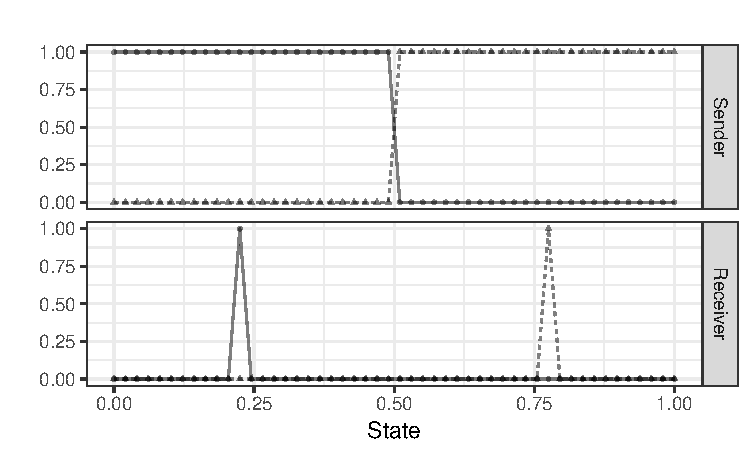
\includegraphics[width=\textwidth]{Rplot-example-strict.pdf}
    \caption{Crisp}
    \label{fig:example_stratsA}
  \end{subfigure}
  \hfill
  \begin{subfigure}[]{0.45\textwidth}
    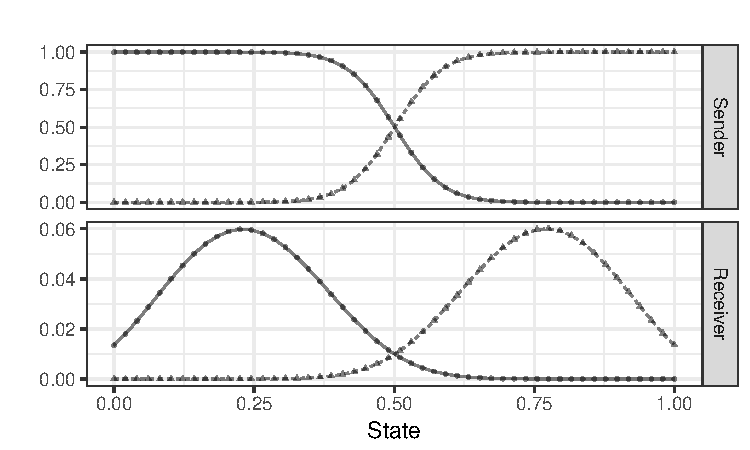
\includegraphics[width=\textwidth]{Rplot-example-vague.pdf}
    \caption{Vague}
    \label{fig:example_stratsB}
  \end{subfigure}

  \caption{Example strategies for a state space with 50 states. Each line corresponds to a message. For the sender, it plots for each state the probability that the message is used. For the receiver, it plots for each state the probability that the response is that state, given the message.}
  \label{fig:example_strats}
\end{figure}

In an abstract setup, using 50 states uniformly distributed over the unit interval and two possible messages, such an optimal language looks like what we see in Figure~\ref{fig:example_stratsA}: the probability that the sender uses one message decays sharply from 1 to 0, and increases sharply from 0 to 1 for the other message; the response of the receiver for each message is a degenerate distribution over the state space.
The sender/receiver strategy pairs that we are looking for look more like Figure~\ref{fig:example_stratsB}, where the sender's choice of message to use is characterized by a smooth transition, and the receiver strategy assigns a positive probability to more than one state for each message.
The particular shapes of these strategies are not important to characterize a vague signal use.
What is important is that the transition is smooth and monotonous for both players.
This means that, for some states in the middle of the state space, there is uncertainty as to which message will be used, whereas for states in the extremes this is as good as certain.

The interpretation of this uncertainty will be different depending on the interpretation of the model.
If we see it as an explanatory model of how two agents play the game, we can see it as randomization.
If we interpret the model as descriptive, it simply represents expected behavior in a manner agnostic to the underlying mechanisms.
A third option is to see probabilities as capturing relative numbers in a population of agents.
For example, if the sender strategy assigns a probability of $0.4$ of message $m$ being sent for state $t$, this would mean that $40\%$ of the population uses that message for that state, while $60\%$ uses the other.
This latter option leaves open the possible interpretation that each agent commands a crisp language and vagueness is only a population-level effect.
However, given the level of abstraction of the description so far, none of this is necessarily implied by the model.
Our question is thus what additional modifications to sim-max games are sufficient for the optimal languages to be more like Figure~\ref{fig:example_stratsB}, rather than like Figure~\ref{fig:example_stratsA}.
%Let's look at some proposals in the literature.

% \subsection{Bounded rationality}
\textcite{franke_vagueness_2011} make two suggestions of how vagueness in a signaling game can be boundedly rational, \emph{i.e.}~how vagueness could arise as a consequence of cost-saving limitations in the cognitive capacities of instrumentally rational agents.
The first proposal is called limited memory fictitious play (LMF) and models agents playing a sim-max game where their ability to recall past interactions with others is limited to a certain number.
For a given interaction, each agent uses his limited memory of the other agent's past behavior to estimate the other's strategy.
Each agent plays an instrumentally rational best response (given the utility function) to their estimate of the other's strategy.
In order to study the evolution of strategies in repeated interaction, the authors model several individual agents in actual play.
What they observe is the emergence of vague signaling at the level of the population, \emph{i.e.}~population averages of individual strategies exhibit the characteristics of a vague language as characterized before.
However, each agent still commands a crisp language, which is inadequate if the intention is to capture how vagueness presents itself in human languages.

In order to overcome this limitation, \citeauthor{franke_vagueness_2011} make another proposal using the notion of a quantal response equilibrium (QRE).
The idea, inspired by experimental psychology, is to model the choice of best response as stochastic rather than deterministic.\footnote{Probabilistic choice rules are also the source of vagueness in recent accounts by \textcite{LassiterGoodman2015:Adjectival-vagu} and \textcite{QingFranke2014:Gradable-Adject}.} 
A prominent explanation for such soft-max or quantal choice behavior is that agents make small mistakes in the calculation of their expected utilities \parencite{Train2009:Discrete-Choice}. 
They still choose the option with the highest expected utility, but each assessment of the expected utilities is noise perturbed.
This, in turn, may actually be boundedly rational since the calculation of expected utilities relies on assessing stochastic uncertainty, which in turn may be costly to calculate precisely. 
Choice based on a few samples from a distribution can be optimal if taking more samples or other means of better approximating degrees of uncertainty is resource costly \parencite[\emph{e.g.}][]{VulGoodman2014:One-and-Done-Op,SanbornChater2016:Bayesian-Brains}.
The degree to which agents tremble in the calculation of expected utilities and therefore deviate from the instrumentally rational behavior can be characterized by a parameter.
\citeauthor{franke_vagueness_2011} find that for low values of this parameter, only babbling equilibria are possible, where sender and receiver simply randomize, respectively, message and interpretation choice uniformly.
Above a certain value of the parameter, other equilibria of the kind described in the beginning of this section arise, where agents communicate successfully, though not perfectly, using fuzzy strategies similar to the ones depicted in Figure~\ref{fig:example_stratsB}. However, it is not clear whether soft-max choices capture the right stochastic trembles in decision making as they would arise under natural sources of uncertainty about the context \parencite[see][]{franke_vagueness_2017}.

% \subsection{Generalized reinforcement learning}
Cailin O'Connor~\parencite*{oconnor_evolution_2014} proposes a way in which vagueness could be expected to evolve as a side-effect of a particular type of learning process.
She studies sim-max games driven not by rational choice dynamics, but by generalized reinforcement learning (GRL), a variant of Herrnstein reinforcement learning (HRL)~\parencite{roth_learning_1995}.
In HRL, agents learn to play a signaling game by strengthening particular choices (of messages for the sender, of responses for the receiver) proportionally to how successful those choices prove to be in an interaction.
O'Connor's proposal is to model generalization as the propagation of reinforcement to nearby states, where ``nearby'' is defined in terms of distance in state space.
For example, if a sender was successful in using message $m$ for state $t$, he will not only positively reinforce that choice of message for $t$, but also for states similar to $t$.
This is done to a degree that is proportional to the similarity between $t$ and other states.
The dynamics also gives rise to vague signaling of the kind we are looking for.

But why should agents evolve to generalize?
%First, it is not argued that vagueness in itself is beneficial, but that it is a by-product of a learning mechanism.
O'Connor suggests that, despite a vague language having lower expected utility than a precise one, the learning mechanism that induces vagueness does have evolutionary advantages, though less obvious ones (see \textcite{oconnor_evolving_2015} for the detailed argument).
Considerations of optimality of strategies, for example by analysing evolutionary stable states, are typically made in terms of hypothetical atemporal comparisons of expected utility.
However, GRL has an interesting property in comparison with more strict learning mechanisms: it achieves higher payoffs in a shorter period of time.
In a naturalized evolutionary setting, where we care about bounded rationality in a multi-context environment, learning speed is an advantage which should also be taken into account.
Imagine an initial population of agents with random strategies, some using GRL and others using classical HRL to adapt to each other.
Although the latter type of agent can hypothetically develop a precise and more efficient signaling system, agents using GRL would coordinate on vague signaling strategies with high (though not optimal) expected utility sooner than agents using HRL.
In such a scenario, they could drive the other agents to extinction before the latter had time to achieve coordination and reap the benefits of a more precise signaling system.


But would such a language be stable?
In terms of evolutionary game theory, one could argue that a small enough group of mutants playing a precise signaling system could later invade a population of vague signalers.
There is, however, an additional advantage to the generalized learning that is relevant here, namely the ability to adapt to a changing environment.
Analysis of a game in terms of evolutionary stable states works well if we assume that the environment where the agents interact remains static.
However, in a more realistic setting this is not the case.
In a dynamic game with a variable environment, an ability to converge faster could give an evolutionary advantage over strict learning rules: as soon as the state space or the utility function change, GRL would quickly adapt and again potentially drive more strict learning mechanisms to extinction because of its short-term gains.


% \subsection{Noisy perception}
\textcite{franke_vagueness_2017} study a variant of the replicator dynamics that is motivated by perceptual limitations.
Assuming that agents do not have perfect perception, there will always be a possibility that senders confuse states and receivers mix up responses.
Furthermore, it seems reasonable to assume that this state confusability is proportional to state similarity, \emph{i.e.}~that the more similar two states are, the more likely it is that they will be mistaken for each other.
Incorporating these considerations into a derivation of the replicator dynamics based on imitation processes, they develop a variant of the dynamic that also induces vague signal use of the kind we expect here.
The consequence is very similar to that of the GRL model discussed above, in that the way the behavior for a given state is updated takes into account the behavior of similar states, proportionally to their similarity.
Given the known relation between reinforcement learning and the replicator dynamics~\parencite{Beggs2005}, it is actually quite plausible that the two are tightly related (although this would need to be formally demonstrated).
The account is, furthermore, interpretable at a lower level of rationality, given that the replicator equation is suitable to represent biological processes of natural selection.

The motivation underlying this model of vague signaling is still one of inevitability.
A vague strategy is not claimed to have higher expected utility than a crisp one.
However, the authors observe an effect similar to that pointed out by~\citeauthor{oconnor_evolution_2014}: signaling converges faster and more often in scenarios where there is some degree of state confusability.
Furthermore, they observe one additional potentially beneficial property.
By running several rounds of simulation for each parameter set, they can measure for each group of results how close resulting strategies are to each other, and how they would fare playing against one another.
The results show that the within group distance between strategies becomes smaller with growing confusability, and the within group expected utility is actually higher for strategies evolving under a certain degree of state confusion.
Thus, some amount of uncertainty seems to promote more homogeneous populations of signalers that are better at achieving cooperation within a group.
%In this picture, vagueness is the natural and unavoidable consequence of perceptual limitations, but may still contribute to the overall boundedly rational character of language if we take multiple contexts of learning into account.

% \subsection{Aggregation from multiple senders}
Finally, \textcite{lawry_vagueness_2017} explore the potential benefits of vagueness in variations of a sim-max game with multiple senders and one receiver.
Although the models considered are not explicitly identified as sim-max games, they are equivalent in the relevant aspects.
They are signaling games where senders have private knowledge of a given state $x$, each sends a message to the receiver, which then selects an estimate $y$ of the original state.
Although the authors do not define a utility function, their analysis evaluates the models in terms of the expected error between the estimate and the original state, defined as $(x-y)^2$.
Better models have lower expected error, thus one could say that the objective is to minimize this function, which would be equivalent to maximizing its inverse.
The game could then be seen as a sim-max game with multiple senders and negative squared difference as utility function.

Unlike the models discussed so far that introduce minimal constraints to a dynamic and study the strategies that emerge out of an evolutionary process, \citeauthor{lawry_vagueness_2017}' approach is mostly static and analytical.
They consider several possible sender strategies, with and without uncertainty, and calculate if and when sender and receiver achieve better transmission accuracy, \emph{i.e.}~smaller expected error between original state and receiver estimate.
Senders without uncertainty have a strategy that boils down to what is represented in Figure~\ref{fig:example_stratsA}: they split the state space according to a fixed threshold, switching from using one message to another abruptly.
The model for the other type of sender is similar, but assumes that there is uncertainty regarding the value of the threshold, representing it as a uniformly distributed random variable.
What results from this in terms of sender strategy is also a smooth transition between the use of two messages.%
\footnote{Unlike what we see in Figure~\ref{fig:example_stratsB}, it is a linear transition. This is certainly connected with the choice of modeling the uncertain threshold as uniformly distributed. We speculate that another choice of distribution, such as for example a normal distribution, could yield something similar to Figure~\ref{fig:example_stratsB}.}%
The receiver strategy is not inherently vague for either type of sender, it merely aggregates the messages received to provide an estimate of the original state using a simple arithmetic mean.

The authors analyze a number of variations of this model.
For a model with one sender, results are consistent with Lipman's~\parencite*{lipman_why_2009} in that strategies without uncertainty lead to more accurate communication.
For models with two messages and more than one sender, the expected error is a strictly decreasing function of the number of senders, and above a certain number of senders, strategies with uncertainty actually achieve lower expected error than crisp ones.
This minimal number of senders from which vagueness surpasses sharpness is a decreasing function of the number of messages, \emph{i.e.}~whereas at least 8 senders are needed if the number of messages available is 2, this number lowers to 5 for 3 messages, 4 for and 5 messages, and 3 for more than 6 messages.
If random errors are introduced between the choice of the sender and the message that reaches the receiver, increasing the number of senders can compensate for the noise, to a certain extent.
Results are mixed when dropping the assumption of uniform priors for the state space.

These results are interesting since they reveal scenarios where vague strategies have an advantage over strict ones, even in a setting of game-omniscient strategic agents.
The approaches discussed so far argue that vagueness is the inevitable byproduct of either cognitive limitations or a particular learning mechanism in the context of other learning mechanisms, which still leaves the idealist\footnote{In an ordinary, non-philosophical, sense.} some room for speculation.
In the models of \citeauthor{franke_vagueness_2011}, the idealist could argue that higher rationality (better memory, or more reliable computation of expected utilities) would lead to more precision.
\citeauthor{oconnor_evolving_2015}'s learning strategy could theoretically be dominated by a process with higher strategic rationality, like best response dynamics~\parencite{gilboa_social_1991}.
A combination of both would hypothetically lead to a better outcome in the scenario of \citeauthor{franke_vagueness_2017}.
\citeauthor{lawry_vagueness_2017} give us something that holds even if the idealist is unwilling to acknowledge the constraints that pervade our finite existence.
Whether the strategies proposed by the authors would be the ones to evolve\footnote{The authors' analysis is a static one. Despite the advantage of the proposed vague strategies against strict ones in certain settings, one cannot know whether other strategies of higher accuracy would not be possible in those same settings without studying some dynamics in an evolutionary context.}, is something that is, however, open for debate.


\section{The ecology of vagueness}
\label{sec:ecology-of-vagueness}

Arguments of the kind presented by Lipman~\parencite*{lipman_why_2009}, that vague signal use is suboptimal when compared to a crisp one, work under a number of various assumptions.
Part of the picture formed by these assumptions is a highly idealized conception of the agents involved and of the context in which they develop and use signals.
These idealizations probably originate, via game theory, from the conception of rationality of traditional theoretical economics.
Herbert A.~Simon describes this picture as follows:
\begin{quote}
Traditional economic theory postulates an ``economic man,'' who, in the course of being ``economic'' is also ``rational.''
This man is assumed to have knowledge of the relevant aspects of his environment which, if not absolutely complete, is at least impressively clear and voluminous.
He is assumed also to have a well-organized and stable system of preferences, and a skill in computation that enables him to calculate, for the alternative courses of action that are available to him, which of these will permit him to reach the highest attainable point on his preference scale.%
~\parencite[99]{simon_behavioral_1955}
\end{quote}
%This ``economic man'', a game-omniscient and highly strategic, instrumentally rational agent, seems to have survived almost unscathed to now populate most game theoretic models of language and signaling.
Both Simon and Lipman call for this picture to be revised, and this is what the proposals surveyed here all do.
In order to account for vagueness in natural language in the context of these models, they peel away from this idealized picture and bring some of these assumptions down to earth.
In the process, they point to ways in which we, as language learners and language users, are finite beings finding ways to cope with a highly complex and dynamic environment:
\begin{enumerate}
\item Our existence is temporally finite; language does not have an infinite amount of time to evolve, nor can it take an infinite time to be learned. The faster a language can start being useful, the better;
\item Language learning through experience has to rely on a limited number of observations. Not only is the state space typically much larger than what one can survey in sufficient time, it is even potentially infinite and constantly changing;
\item A corollary of the former is that there will always be heterogeneity in a population of language learners, at the very least in their prior experience, since each agent will have relied on a different set of observations. Furthermore, this information is not directly or fully accessible to others;
\item Given that an agent is almost always learning and using language in a population of other agents, there are also various potential sources of linguistic input the agent is constantly integrating in his practice.
\end{enumerate}
All of these observations support the weakening of the modeling assumptions.
% If we take these points seriously, we have to concede that it is almost inevitable that uncertainty gets introduced at almost all levels of language learning and language use.
% In the context of a signaling game, we can expect uncertainty about priors, observations, utilities, behavior of other players, and more.
% This is true both from the perspective of the modeler, as from the perspective of the agents involved, supporting the motivation to take it into account in our modeling efforts.
The research surveyed here shows us some examples of assumptions which, when weakened, make vague signal use a natural outcome of certain evolutionary dynamics.
% That includes considering various mechanisms that can lead to vague use of messages in certain signaling games: cognitive limitations like a finite memory or the inability to always calculate the absolute optimum choice to make; learning mechanisms that compensate for the finiteness of experience through generalization based on similarity; and imperfect senses that allow for the possibility of stimuli to be confused, etc\todo{fit Lawry and James plus referential games stuff}.
But it gives us even more.
It suggests ways in which the mechanisms that lead to vagueness can have positive effects that are extremely important in the context of the points just enumerated.
We learned from \citeauthor{oconnor_evolution_2014} and \citeauthor{franke_vagueness_2017} that vague languages are quicker to converge and adapt, which is valuable given the finite and dynamic character of our experience (point 1).
\citeauthor{oconnor_evolving_2015} also showed how generalization, an invaluable feature of any procedure for learning from a limited number of observations (point 2), leads to vagueness.
We also learned from \citeauthor{franke_vagueness_2017} that state confusability, a mechanism thats leads to vague signal use, can have a homogenizing effect on vocabularies, potentially compensating for the heterogeneity of agents' experiences (point 3).
\citeauthor{lawry_vagueness_2017} demonstrated the benefits of strategies that incorporate uncertainty, leading to vagueness, in language games where agents need to aggregate information from various sources (point 4).
%Trying to answer the question of ``Why is language vague?'', is important to force us to recognize those aspects of language and the world that are easily forgotten when idealizing the subject matter.
%The finiteness of human experience, the dynamic nature of the world, and the communitarian context of language use and development, these are things we need to keep in mind lest we end up with inadequate models of language and meaning.
% Wittgenstein put it better:

What do these observations tell us about rationality?
% The replicator equation lends itself to an interpretation where agents could be said to be devoid of rationality, procedural or instrumental.
% This is the case where we see the equation as purely descriptive of a population of agents with hardwired behaviors, where the most successful strive and the least successful die off.
% In such an interpretation there is no room for questions regarding the rationality of vagueness.
% Another possible interpretation is that of a population of agents learning by imitation.
GRL~\parencite{oconnor_evolution_2014} and the work of~\textcite{franke_vagueness_2017} both assume a picture of agents with a basic level of instrumental rationality, possibly limited awareness of the game and a lack of strategic capabilities, adapting their behavior with only short-term gains in sight.
%Under the standard assumptions, even agents with such limited rationality would evolve crisp signaling in sim-max games.
These approaches introduce constraints on agent behavior or information processing that prevent the evolution of crisp signal use.
But a crisp language would still have a higher expected utility than the evolved strategies.
Agents in those models seem to be only as rational as the modelers allow them to be.
Despite the plausibility of the mechanisms proposed (limited memory, imprecise calculation of expected utilities, generalization, state confusability), the results of these models feel somewhat bittersweet because of the hypothetical possibility of an ideal strategy, seemingly barred from the agents in an artificial manner.
Couldn't a more rational agent evolve and drive the system into crisp signal use?
Aren't we, human beings, that kind of agent?

Perhaps a deeper understanding of vagueness and the reasons for its pervasiveness in natural language are to be found only when we broaden the scope of the models employed.
%We call this the \emph{ecology} of vagueness.
All the models discussed so far explore evolutionary dynamics for one homogeneous population playing one game.
Different types of agents and different game setups are considered, but each of these different possible scenarios is always tested separately.
We see at least two ways in which one could have a more ecological perspective.
The first is to think about meaning and vagueness with a more Wittgensteinian perspective.
We can see each signaling game as embodying a particular language game.
In Wittgenstein's picture of language, however, we do not play only one language game in our existence; there is a plurality of them and which one an agent is engaged in at a particular moment is never clearly identified, neither are the exact benefits one might take out of it by choosing a certain behavior over another.
These are furthermore not fixed in time; old language games fall out of fashion or stop being useful, and new ones emerge all the time~\parencite[see][and in particular \S 23]{wittgenstein_philosophical_1953}.
We could look for rationality at several levels in this pluralistic picture.
Firstly, as before, there is the actual behavior of a single agent in each actualized language game.
As mentioned above in connection the soft-max choice function used by \textcite{franke_vagueness_2011}, behavior that strictly maximizes expected utility under uncertainty may be resource heavy, so it might be compatible with local strategic rationality that agents' production choices are stochastic.
%% \mf{mention ``bounded rationality'' here}
Secondly, if we look at behavior across many game types and contexts, there is also the level of an agent's internal theory of how words and phrases are likely to be used (or even normatively: how messages should be used), conditional on a given context.
Notice that a single agent's rational beliefs about linguistic practices or linguistic meaning may well have to reflect the actual stochasticity: under natural assumptions about information loss, the best belief for prediction matches the actual distribution in the real world \parencite[\emph{e.g.}][]{VehtariOjanen2012:A-survey-of-Bay}.
In sum, both at the level of behavior and at the level of beliefs about use or meaning, we should expect to find vagueness.
Still, despite the natural vagueness, there does not seem to be anything fundamentally missing or conceptually incoherent in a naturalistic, rationality- or optimality-driven explanation of what each agent is doing or what each agent beliefs about language, use and meaning.

Another way to go beyond locality is to work with more heterogeneous population models.
The mechanisms that lead to vague signal use, as~\textcite{oconnor_evolution_2014} and~\textcite{franke_vagueness_2017} stress, have the aforementioned important advantages of faster speed of convergence, higher flexibility, and homogenization.
The argument goes that these side-effects, by temporarily enabling a higher expected utility, could allow a population using some generalization (or affected by some imprecision) to take over.
However, despite its intuitiveness the argument is based on comparing isolated runs of different dynamics.
The models do not allow the hypothesis to be tested, because they do not accommodate different populations evolving together.
%These advantages matter, especially in the complex, dynamic context of real language use.
%Limits on memory and precision in the calculation of complex probabilistic beliefs may have a reduced metabolic processing cost.
%One would thus like to say that using a strategy that promotes those characteristics without a significant loss of expected utility is certainly a rational choice.
%But in order to be able to say that in the context of the model, we need either a notion of rationality that goes beyond local maximization of expected utility, or a notion of expected utility that incorporates other dimensions.
%It is in this sense that these explanations tie in with a notion of bounded ecological rationality.
%
%For more complex agents, the story is potentially more nuanced.
%Consider an agent that has awareness that something like a game is being played, some estimate of the potential payoff involved, ability to gauge other players' expected behaviors, and the capacity to think strategically.
%Is it rational for a sender to use a message in a crisp way, splitting the state space as if a strict threshold existed between the use of one term and the other?
%In a scenario where the agent's ability to make the optimal choice is bounded, such as in the models of~\textcite{franke_vagueness_2011}, the agent is again doing the best he can given the constraints imposed on him.
%\textcite{lawry_vagueness_2017} draw attention to another option we need to consider: such agents could opt to ignore their limitations and external sources of uncertainty and use a crisp strategy regardless.
%The authors' analysis shows that such an approach would be irrational in a number of different scenarios, even in the narrow interpretation of rationality as local utility maximization.
%But even in other scenarios, we could again argue that, if we broaden our notion of rationality, it would be less rational to use a crisp strategy rather than one that incorporates at least some source of uncertainty.
%A crisp strategy for a particular game would, in most realistic scenarios, take more time to achieve convergence, be less adaptable to changes, less easy to reuse in other similar games, and less able to foster cooperation with a bigger group of agents.
%Though potentially a locally rational choice, it might thus not be globally optimal.
%
%In the context of signaling games, thinking about vagueness from a more ecological perspective means broadening our models to incorporate more diversity and allow the study of additional interactions within the model.
%There are many ways in which this can be done.
In the remainder of the paper we propose a way to do this for the model of~\textcite{franke_vagueness_2017}.
We introduce two variations of a multi-population model of the imprecise imitation dynamics, where populations characterized by different imprecision values interact and evolve together.
Using this model, we can better see under which conditions the hypothesized advantages of some imprecision can lead to the evolution of vagueness.

%We believe these considerations are, again, very much in line with Wittgenstein's later philosophy:
%\begin{quote}
%The more closely we examine actual language, the greater becomes the conflict between it and our requirement.
%(For the crystalline purity of logic was, of course, not something I had discovered: it was a requirement.)
%The conflict becomes intolerable; the requirement is now in danger of becoming vacuous.
%– We have got on to slippery ice where there is no friction, and so, in a certain sense, the conditions are ideal; but also, just because of that, we are unable to walk.
%We want to walk: so we need friction.
%Back to the rough ground!%
%~\parencite*[\S 107]{wittgenstein_philosophical_1953}
%\end{quote}
%This seems like a very clear call for what we are arguing here.
%But are we exposing ourselves to ``philosophical disease'' by following a ``one-sided diet''~\parencite*[\S 593]{wittgenstein_philosophical_1953} when looking only at sim-max games?
%In the spirit of Wittgenstein's pluralistic picture of language, we would like to reflect on vagueness in one more type of signaling game and speculate on the impact of plurality for vagueness.


%\section{Vagueness in multiple reference games}
%\label{sec:referential-vagueness}
%
%The type of linguistic interaction captured by a sim-max game has its own particular scope.
%There is a fixed prior, a fixed utility function and a fixed similarity measure between states.
%If the sender observes a state $t$ and the receiver guesses state $t'$ the utility of that interaction is proportional to the similarity between $t$ and $t'$.
%Here is a natural example of a situation captured by a sim-max model: Kiki wants Bubu to draw her dissertation cover in a particular shade of blue; the closer Bubu's color choice matches Kiki's idea, the better. Here Kiki wants to \emph{describe} the color for Bubu to pick out or realize from the whole set of possibilities.
%It's a natural thing to want to do with language.
%But other types of communication with vague and contiguously variable properties are possible.
%A \emph{reference game} is a model of a situation in which the speaker has a particular object in mind and uses a description in order for the receiver to pick this object and no other object.
%One crucial difference with sim-max games is that close will not be close enough: if Kiki needs a long nail, a nail a little longer or shorter may be good enough; but if Bubu needs the long, slightly bend nail with the flat top (which she previously disassembled from her art installation), no other nail will do.
%
%Interestingly, referential communication can take place under a plethora of different epistemic conditions.
%A lot of modeling work considers \emph{reference games without displacement} where sender and receiver communicate about a context, i.e. a set of objects, which is immediately accessible in their direct perceptual environment \parencite[\emph{e.g.}][]{BaronchelliGong2010:Modeling-the-Em,Franke2012:Scales-Salience,Franke2012:On-Scales-Salie}.
%Agents may make mistakes about observing exactly how blue or long etc.~a particular object is, but there is no further fundamental uncertainty about the context.
%This, of course, need not be so. \textcite{lipman_why_2009} and \textcite{Deemter2009:Utility-and-Lan}, for example, consider \emph{reference games with displacement}.
%Kiki asks Bubu to fetch the red book from the library.
%No other book than the one Kiki needs will serve.
%When Kiki describes the book, the perceptual context in which Bubu must make her choice is not co-present to Kiki at the time of speaking.
%Yet other situations are imaginable.
%In \emph{reference games with partial uncertainty}, for instance, interlocutors may know that they have shared and immediate access only to a subset of the objects in the context, but be uncertain about whether the co-player sees any other objects.
%This is the set-up for the widely-used director task in psycholinguistics \parencite[\emph{e.g.}][]{KraussGlucksberg1977:Social-and-nons,Keysar2000,KeyzarLin2003:Limits-on-Theor}.
%
%What would a rational agent do in repeated reference games?
%Take a universe in which agents play repeated reference games without displacement.
%A single game has sender and receiver both flawlessly perceive a context of $k$ objects (with $k$ possibly randomly drawn for each encounter); each object has its individual features, e.g., drawn from a rich multidimensional feature space of continuously variable properties \parencite[\emph{e.g.}][]{Franke2012:Scales-Salience,Franke2012:On-Scales-Salie}.
%The sender chooses a message $m$ for the target object $t$, but she can condition her choice on the current context $c$.
%Likewise, the receiver chooses a referent $t'$ from the available objects in $c$, again conditional on $c$.
%But if agents play many such reference games with different contexts $c$ and $c'$, strategic and instrumental rationality of local choices in $c$ and $c'$ is not enough to guarantee that agents' beliefs and behavior in $c$ have any relation to their beliefs and behavior in $c'$.
%An agent could use a certain signal to denote, say, the tallest object in every context with between five and twelve objects or when the number of objects is a prime number, but use the same signal for the darkest object in all other contexts.
%In other words, neither rationality of choice in a fixed context nor evolutionary adaptation to each single context entails a natural, globally consistent behavior across multiple contexts.
%The situation only gets worse if we want to have agents use the same expressions in a consistent way also across different types of reference games, with possibly different epistemic conditions.
%
%The picture just sketched neglects learning from observation, as well as generalization across contexts.
%For strategic and instrumentally rational agents, we need to consider also the ability to learn from previous experience and to generalize from the past to the future.
%For evolutionary adaptation, the story so far misses the key fact that languages and practices have to be learnable in appropriate time from the actual observables, lest what is learned and further transmitted will simply be a different language or practice \parencite[\emph{e.g.}][]{KirbyGriffith2014:Iterated-Learni}.
%But even if every language learner in history had been perfectly rational, it is extremely unlikely, as was discussed in the previous section, that anyone ever succeeded in reducing all uncertainty about language use and say with confidence: this is the threshold that truly separates heaps from non-heaps no matter what.
%For one, there may simply not be enough time in the lifespan of a rational learner to observe enough instances of language use for certainty about crisp denotations.
%For another, what needs to be learned likely changes over time.
%The optimal use for gradable properties hinges crucially on the prior over states \parencite[\emph{e.g.}][]{Franke2012:Scales-Salience,Franke2012:On-Scales-Salie,QingFranke2014:Gradable-Adject,LassiterGoodman2015:Adjectival-vagu}.
%If the prior captures real world attributes, such as the probability of an individual's body height, these attributes will not only be hard to know for certain, but they will also vary over time.
%They may also depend on location: do we use our language exclusively in this village (where all heaps are extraordinarily small and people are extraordinarily tall) or do we travel beyond?
%If so, the priors that determine the goodness of a convention for one agent need not be the same as those for another.
%Going beyond the priors for property degrees, the probability of seeing a particular context $c$ in some kind of reference game, is also crucial for determining globally efficient linguistic behavior.
%But here it is even more inconceivable how a rational learner could acquire a fairly confident estimate over how often the upcoming reference games will have a particular context or another.
%The list of sources of natural and seemingly insurmountable uncertainty about the parameters necessary to determine locally or globally optimal strategies is much longer than hinted at here.
%Still, it should be clear enough that a finite existence, a sparse learning input and the inherent fuzziness of the linguistic context itself (its temporal, local and social variability) is not a fault of rationality on the part of the agent, or the mechanism of selection of successful linguistic practices.
%
%What about meaning and vagueness in a universe of multiple language games and heavy uncertainty?
%We do not play only one language game in our existence; there is a plurality of them and which one an agent is engaged in at a particular moment is never clearly identified, neither are the exact benefits one might take out of it by choosing a certain behavior over another.
%These are furthermore not fixed in time; old language games fall out of fashion or stop being useful, and new ones emerge all the time~\parencite[\S 23]{wittgenstein_philosophical_1953}.
%We could look for meaning at several levels in this pluralistic picture.
%Firstly, as before, there is the actual behavior of a single agent in each actualized language game.
%As mentioned above in connection the soft-max choice function used by \textcite{franke_vagueness_2011}, behavior that strictly maximizes expected utility under uncertainty may be resource heavy, so it might be compatible with local strategic rationality that agents' production choices are stochastic.
%% \mf{mention ``bounded rationality'' here}
%Secondly, if we look at behavior across many game types and contexts, there is also the level of an agent's internal theory of how words and phrases are likely to be used (or even normatively: how messages should be used), conditional on a given context.
%Notice that a single agent's rational beliefs about linguistic practices or linguistic meaning may well have to reflect the actual stochasticity: under natural assumptions about information loss, the best belief for prediction matches the actual distribution in the real world \parencite[\emph{e.g.}][]{VehtariOjanen2012:A-survey-of-Bay}.
%In sum, both at the level of behavior and at the level of beliefs about use or meaning, we should expect to find vagueness.
%Still, despite the natural vagueness, there does not seem to be anything fundamentally missing or conceptually incoherent in a naturalistic, rationality- or optimality-driven explanation of what each agent is doing or what each agent beliefs about language, use and meaning.
%
%% Finally, we might be interested in a notion of meaning of language as an abstraction over their users and its use.
%% We might not care about individual agents' behavior and beliefs as much as we care about the meaning of words, expressions and sentences.
%% The questions to address then are probably: what explanatory purpose is a notion of meaning of an abstracted language to play?; if both agents' rational behavior and rational beliefs are plausibly fuzzy, why should a concept of supervening meaning be crisp?; what can be explained only by a notion of meaning that is not vague?
%% \mf{I leave this paragraph in for you to read and ponder, but would recommend to leave it out entirely}
%
%Taken together, when we look at the picture of multiple language games side by side, the question of what rational or optimal behavior is in any one of them, or the question of why human language users do not more closely approximate instrumentally rational or optimal local behavior more closely seem entirely misplaced.
%What seems more pressing is to answer how the interaction of individual learning, individual local optimization and general pressure for successful communication at a cross-situational level lead to the shaping of linguistic practices in an open-ended landscape of language games.
%How to attain locally sub-optimal play in a single language game is not a theoretical puzzle we should take serious, if what really matters is a global multi-game perspective.
%Adopting this perspective does not \emph{solve} the problem of how vagueness is compatible with rationality.
%But it suggest that it might be an inflated issue that we need not or should not worry about, because it will likely not matter in a more realistic and encompassing picture of language, its use and evolution as driven by an appropriate notion of rational choice and evolutionary selection.


\section{Two multi-population models of imprecise imitation}
\label{sec:multi-population-model}
We build upon the model of~\textcite{franke_vagueness_2017}, adding to the imprecise imitation dynamics the support for multiple populations with different imprecision values evolving together.
In order to do this, first we consider that each population evolves according to the imprecise imitation dynamics.
However, we want to model populations that are able to interact with each other.
Therefore, the dynamic needs to be adapted in order to reflect the fact that agents can hypothetically imitate and play against agents with different imprecision levels.
Second, in order to see the impact of the success of different imprecision levels, we need to add another process of selection.
A possible story to motivate these ideas goes as follows: imagine agents who are born with varying perceptual abilities, subsequently learn a signaling strategy by imitation of other agents (either within or across populations), and depending on the success of the strategies they develop are more or less likely to survive and reproduce.
In such setup, we change not only each populations particular strategies, but also the proportion of each population depending on its fitness compared to other populations.

The motivations behind this model are closely related to the ideas behind the theories of kin selection~\parencite{hamilton_genetical_1964} and multi-level (or group) selection~\parencite{wilson_theory_1975}.
These theories build upon the hypothesis that selection acts not only to directly favor genes that result in behaviors that benefit individuals, but also to indirectly favor genes that lead to behaviors that benefit either genotypically (kin) or socially (group) related individuals~\parencite[see][for more details]{okasha_evolution_2006}.
%There are thus two aspects to be considered: for kin selection that would be the direct and indirect effects, and for multi-level selection the within-group and between-group components~\parencite[28--29]{birch_kin_2014}
In our model there is also a similar structure: there is a process of selection of behavior within each population, levels of imprecision are selected across populations based on the strategies they give rise to.
We believe there is an important distinction in that the two selection processes in our model act on different entities, the inner shaping signaling behavior, and the outer selecting levels of imprecision.
In any case, we intend our model to be descriptive rather than causal or explanatory.
That means that we do not want to commit to seeing populations either as kins or as social groups, and use them as merely descriptive abstractions that allow us to capture the hypothetical impact of indirect selection processes%
\footnote{We make this note because of the heated debate between the two theories. See~\textcite{kohn_darwin_2008} and~\textcite{kramer_kin_2016} for more details on that.}%
.

In the following, we lay down the formal details of our model.
Let's start by defining $A$ to be the set of imprecision values considered.
For each value $\alpha \in A$, the proportion of its population is given by $P(\alpha)$, such that $\sum_{\alpha \in A} P(\alpha) = 1$.
The probability that a given agent with imprecision $\alpha$ (or of type $\alpha$) observes $t_o$ when the actual state is $t_a$ is given by $P_{o}^{\alpha}(t_{o}|t_{a})$.
If the same agent intends to realize $t_i$, the probability that he actually realizes $t_r$ instead is given by $P_{r}^{\alpha}(t_{r}|t_{i})$.
Following~\textcite[26]{franke_vagueness_2017}, we can then define the following values.
Probability that $t_a$ is actual if $t_o$ is observed by an agent of type $\alpha$:
$$
P_{\bar{o}}^{\alpha}(t_{a}|t_{o})\propto P_{a}(t_{a})P_{o}^{\alpha}(t_{o}|t_{a})
$$
Probability that a random sender of type $\alpha$ produces $m$ when the actual state is $t_a$:
$$
P_{\sigma}^{\alpha}(m|t_{a})=\sum_{t_{o}}P_{o}^{\alpha}(t_{o}|t_{a})\sigma^{\alpha}(m|t_{o})
$$
Probability that the actual state is $t_a$ if a random sender of type $\alpha$ produced $m$:
$$
P_{\bar{\sigma}}^{\alpha}(t_{a}|m)\propto P_{a}(t_{a})P_{\sigma}^{\alpha}(m|t_{a})
$$
Probability that $t_r$ is realized by a random receiver of type $\alpha$ in response to message $m$:
$$
P_{\rho}^{\alpha}(t_{r}|m)=\sum_{t_{i}}P_{r}^{\alpha}(t_{r}|t_{i})\rho^{\alpha}(t_{i}|m)
$$
These formulations are merely parameterized versions of the single-population model.
They encapsulate calculations that we can use to compute expected utilities and update probabilities for each type.
The latter, however, depend on the types of interaction that we imagine occurring between populations.
In the following sections, we consider two different possibilities.

\subsection{Tight population interaction}
\label{sec:tight-interaction-model}
In a multi-population model with tight interaction between populations, each agent plays with, observes, and potentially imitates any other agent, regardless of their type.
This has an impact on the expected utilities of sender and receiver strategies of each type, and on the update probabilities for those strategies.
Let's start with the expected utilities.
For a sender of type $\alpha$, the expected utility of its strategy $\sigma^\alpha$ against all other receiver strategies $\rho^\star$, is given by:
$$
\text{EU}_{\sigma}^{\alpha}(m,t_{o},\rho^{\star})=\sum_{t_{a}}P_{\bar{o}}^{\alpha}(t_{a}|t_{o})\sum_{\alpha^{\prime}\in A}P(\alpha^{\prime})\sum_{t_{r}}P_{\rho}^{\alpha^{\prime}}(t_{r}|m)U(t_{a},t_{r})
$$
and, for a receiver of type $\alpha$, the expected utility of its strategy $\rho^\alpha$ against all other senderstrategies $\sigma^\star$, is given by:
$$
\text{EU}_{\rho}^{\alpha}(t_{i},m,\sigma^{\star})=\sum_{\alpha^{\prime}\in A}P(\alpha^{\prime})\sum_{t_{a}}P_{\bar{\sigma}}^{\alpha^{\prime}}(t_{a}|m)\sum_{t_{r}}P_{r}^{\alpha}(t_{r}|t_{i})U(t_{a},t_{r})
$$
Expected utilities thus take into account the existence of strategies of other types, and weigh the relevance of each type $\alpha^\prime$ according to its relative proportion $P(\alpha^\prime)$.

Another important value to calculate has to do with the types which agents observe and imitate.
In a model with tight interaction, we imagine this occurring across populations.
Therefore, we can define the probability that a sender of type $\alpha$ observes a randomly sampled agent play message $m$ for observed state $t_o$ as:
$$
P_{o}^{\alpha}(m|t_{o})=\sum_{t_{a}}P_{\bar{o}}^{\alpha}(t_{a}|t_{o})\sum_{\alpha^{\prime}\in A}P(\alpha^{\prime})P_{\sigma}^{\alpha^{\prime}}(m|t_{a})
$$
and the probability that a receiver of type $\alpha$ observes a randomly sampled agent choose interpretation $t_o$ given message $m$ as:
$$
P_{o}^{\alpha}(t_{o}|m)=\sum_{t_{r}}P_{o}^{\alpha}(t_{o}|t_{r})\sum_{\alpha^{\prime}\in A}P(\alpha^{\prime})P_{\rho}^{\alpha^{\prime}}(t_{r}|m)
$$
Again, these calculation incorporate the probabilities that the imitating agent might observe the behavior of an agent of another type $\alpha^\prime$, weighed by its relative proportion.
%
Finally, the update probabilities for a sender strategy of type $\alpha$ at time instant $i+1$ can be given by:
$$
\sigma_{i+1}^{\alpha}(m|t) \propto P_{o}^{\alpha}(m|t)\text{EU}_{\sigma_{i}}^{\alpha}(m,t,\rho_{i}^{\star})
$$
and similarly for a receiver strategy of type $\alpha$ by:
$$
\rho_{i+1}^{\alpha}(t|m) \propto P_{o}^{\alpha}(t|m)\text{EU}_{\rho_{i}}^{\alpha}(t,m,\sigma_{i}^{\star})
$$

These formulations cover the evolution of the particular strategies of each type.
We can think of this as the level of cultural evolution: agents are born with a certain level of imprecision and learn strategies based on the behavior of others.
Alongside this process, we can imagine another level of selection, where agents die and new agents are born.
More successful agents have a higher likelihood of surviving and reproducing, giving rise to more agents with their level of imprecision.
Levels of imprecision are thus subject to an evolutionary dynamic that is indirectly influenced by the cultural dynamic.
Importantly, only the level of imprecision is passed on to new generations under this dynamic, not the actual strategies developed by the agents at the cultural level.

We model this process by changing the proportion of each type $P(\alpha)$ according to the replicator dynamic.
A population of type $\alpha$ consists of agents employing both a sender and a receiver strategy, thus the overall fitness of the population must include the expected utilities of both.
We could imagine this process happening at a different speed than the cultural process, in which case we could have different time scales.
For the sake of simplicity, we choose to have them both happen at each time step, but calculate the changes occurring at this level of selection after the calculation for the other level.
We define the proportion of type $\alpha$ at time step $i+1$ as:
$$
P_{i+1}(\alpha) \propto P_i(\alpha)(\text{EU}_{\sigma_{i+1}}^{\alpha}(m,t,\rho_{i}^{\star}) + \text{EU}_{\rho_{i+1}}^{\alpha}(t,m,\sigma_{i}^{\star}))
$$
In order to additionally account for the fact that strategies are not passed on to new generations, we mix the evolved strategies of a certain type $\sigma^\alpha$ and $\rho^\alpha$ with new random strategies $\tilde{\sigma}^\alpha$ and $\tilde{\rho}^\alpha$ (generated at each time step).
The idea is that, at each time step, a certain percentage of each population will consist of ``newborn'' agents, \emph{i.e.}~agents that haven't yet had time to evolve their strategies.
We define a parameter $\gamma$ that quantifies this percentage, or as we can also call it the birth rate, which we consider to be the same for every population.
This mixing can be described, for a certain time step $i+1$, in the following formulas:
$$
\sigma_{i+1}^{\alpha}(m|t)=(1 - \gamma)\sigma_{i+1}^{\alpha}(m|t) + \gamma \tilde{\sigma}_{i+1}^{\alpha}
$$
$$
\rho_{i+1}^{\alpha}(t|m)=(1 - \gamma)\rho_{i+1}^{\alpha}(t|m) + \gamma \tilde{\rho}_{i+1}^{\alpha}
$$

We performed 25 simulation runs of this model for each of three population scenarios: only one population with $\alpha = 0$ (for reference), two populations with $\alpha \in \{0, 0.05\}$, and three populations with $\alpha \in \{0, 0.05, 0.1\}$.
For each scenario, starting proportions $P(\alpha)$ were equal for each value of $\alpha$.
Given the observations by~\textcite{franke_vagueness_2017} that state space size and tolerance parameter $\beta$ do not result in important qualitative difference, we fixed these values at $n_S = 30$ and $\beta = 0.1$.
We also used a fixed uniform distribution for the priors and a message space with 2 messages.
Each type started with its own randomly generated strategy.
Regarding the duration of the simulations, due to the mixing in of new individuals into the population (birth rate was fixed at $\gamma = 0.05$), the convergence criteria is no longer applicable because each strategy is randomly perturbed at each time step.
Therefore, all simulation runs were stopped after 200 iterations.

The first thing to observe from the simulation results is that the population with no imprecision ($\alpha = 0$) dominated the other populations in every run.
%\begin{sidewaysfigure}
\begin{figure}
  \centering
  \begin{subfigure}[]{\textwidth}
    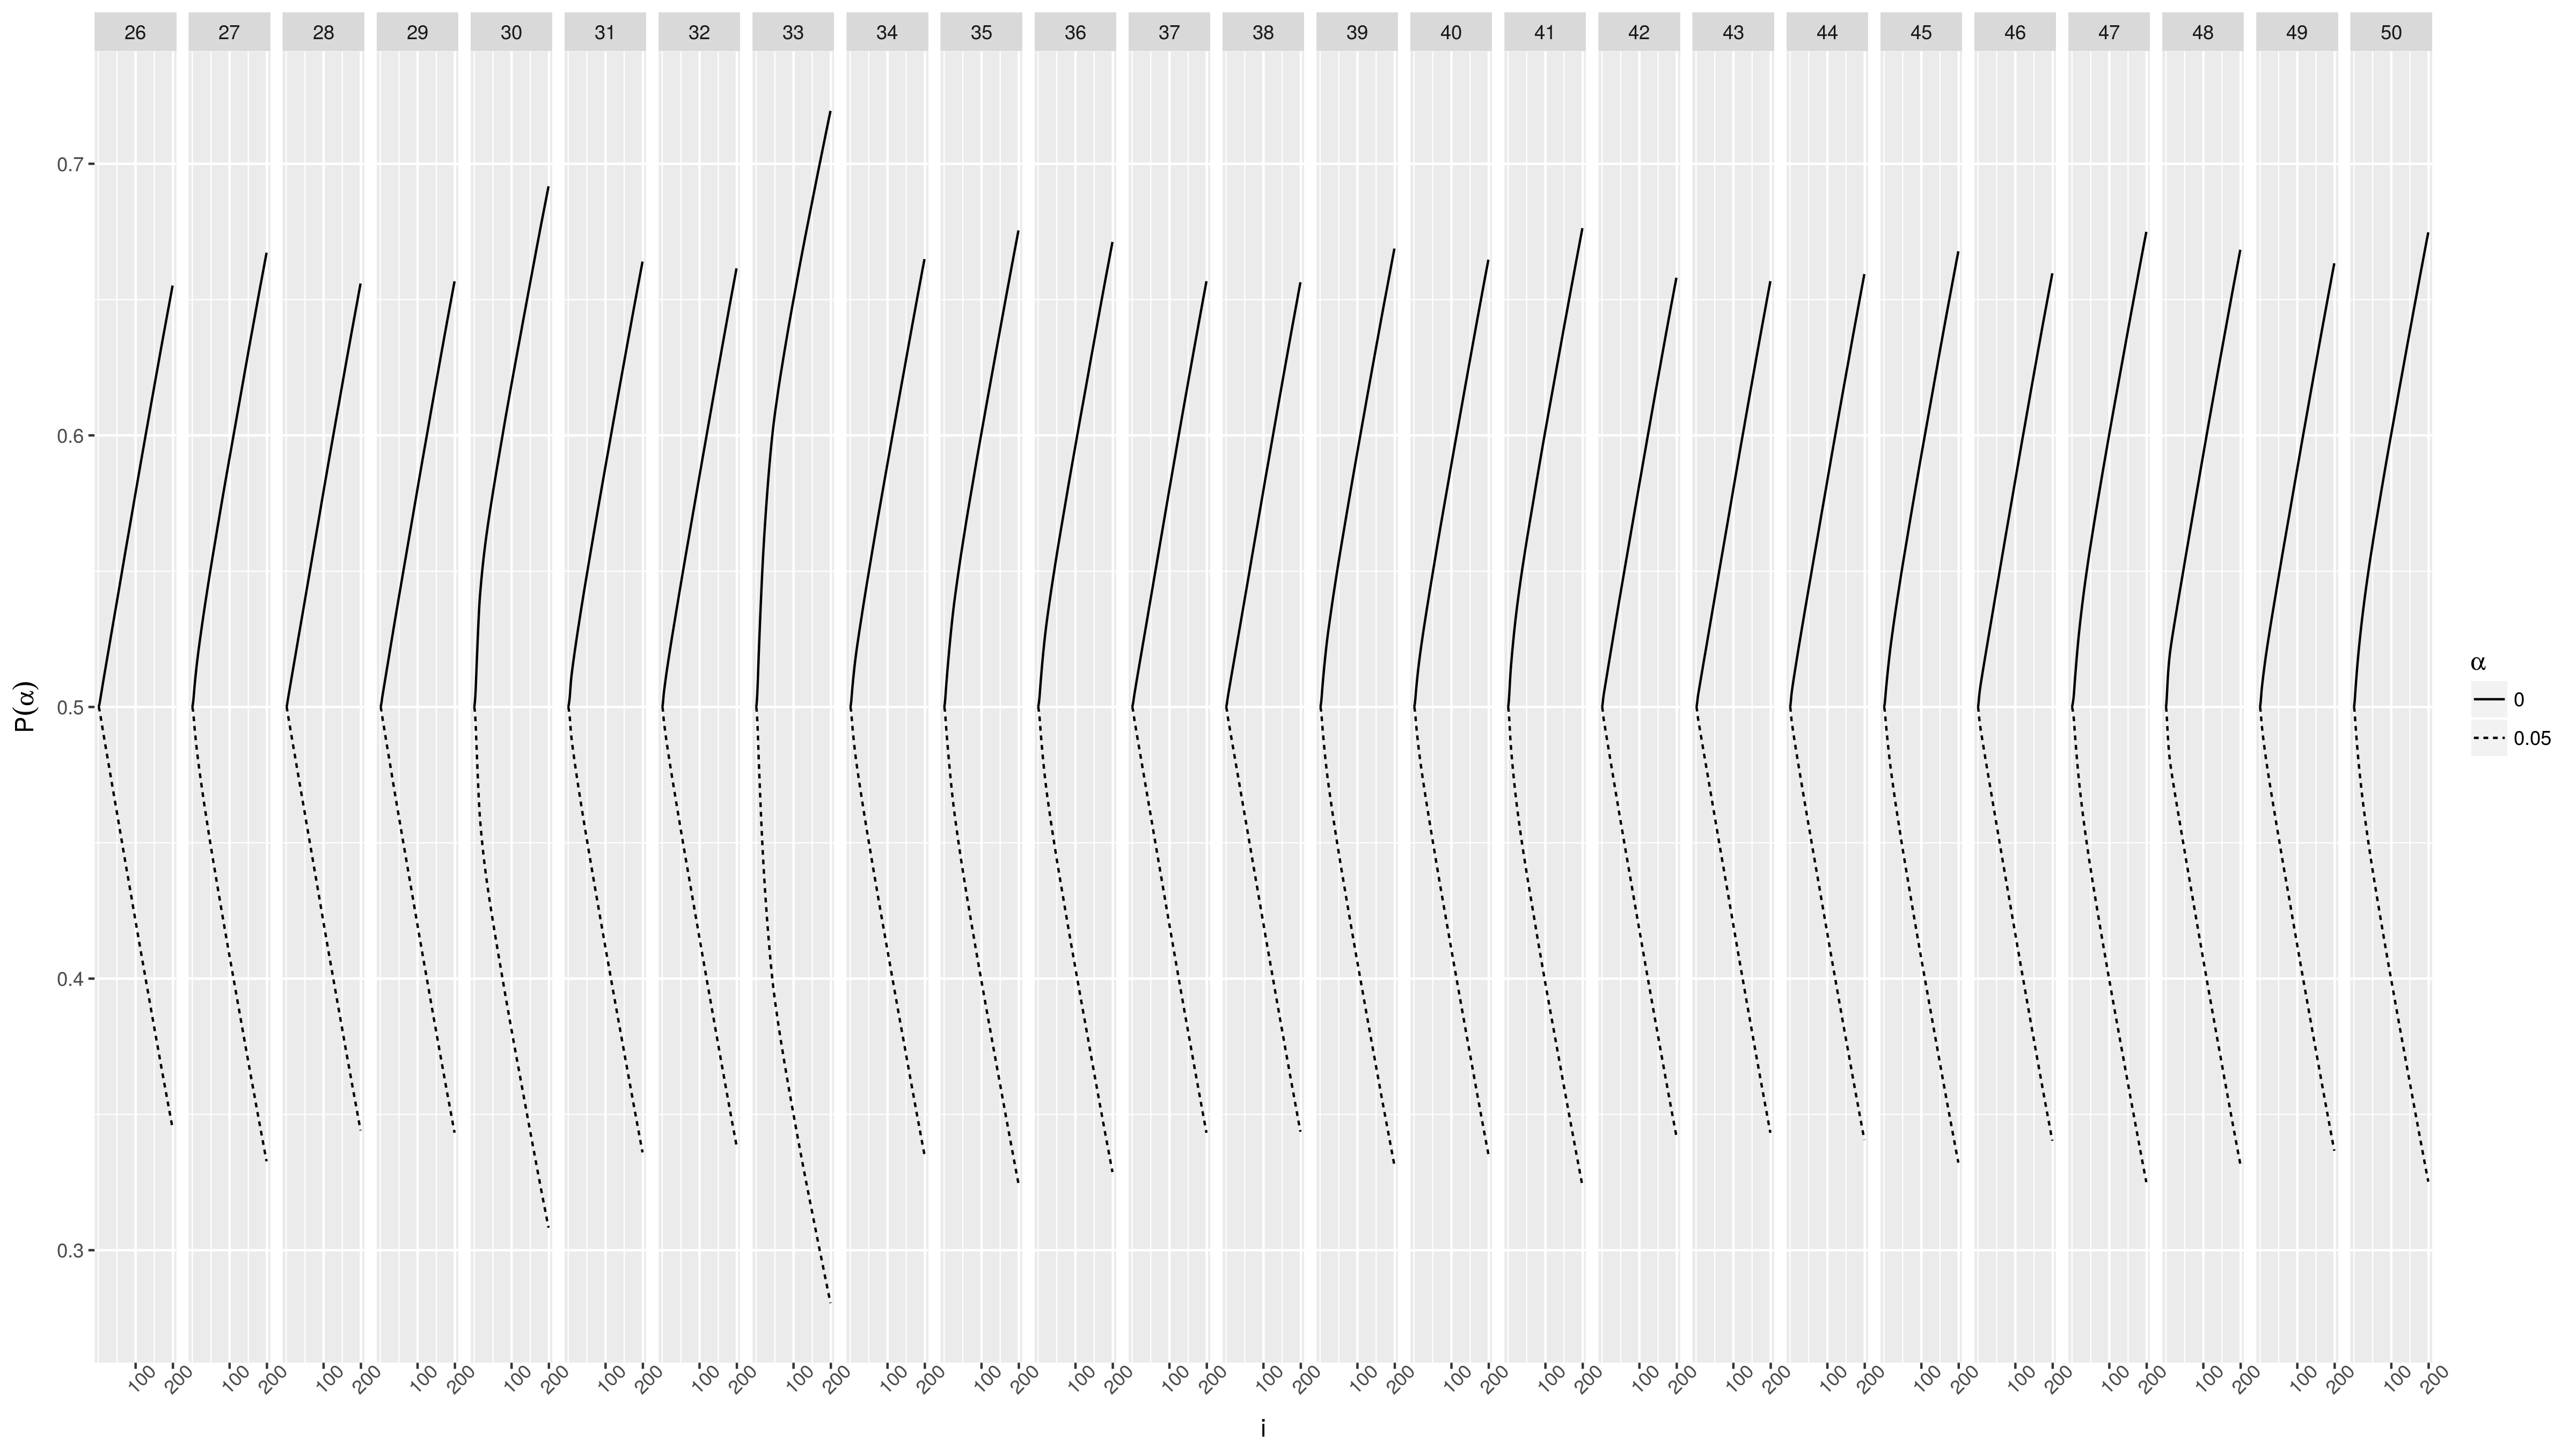
\includegraphics[width=\textwidth]{simulation/results/round-3/plots/proportion-cases-0-005-strong.png}
    \caption{Two populations scenario.}
    \label{fig:proportion-cases-two-tight-interaction}
  \end{subfigure}
  \hfill
  \begin{subfigure}[]{\textwidth}
    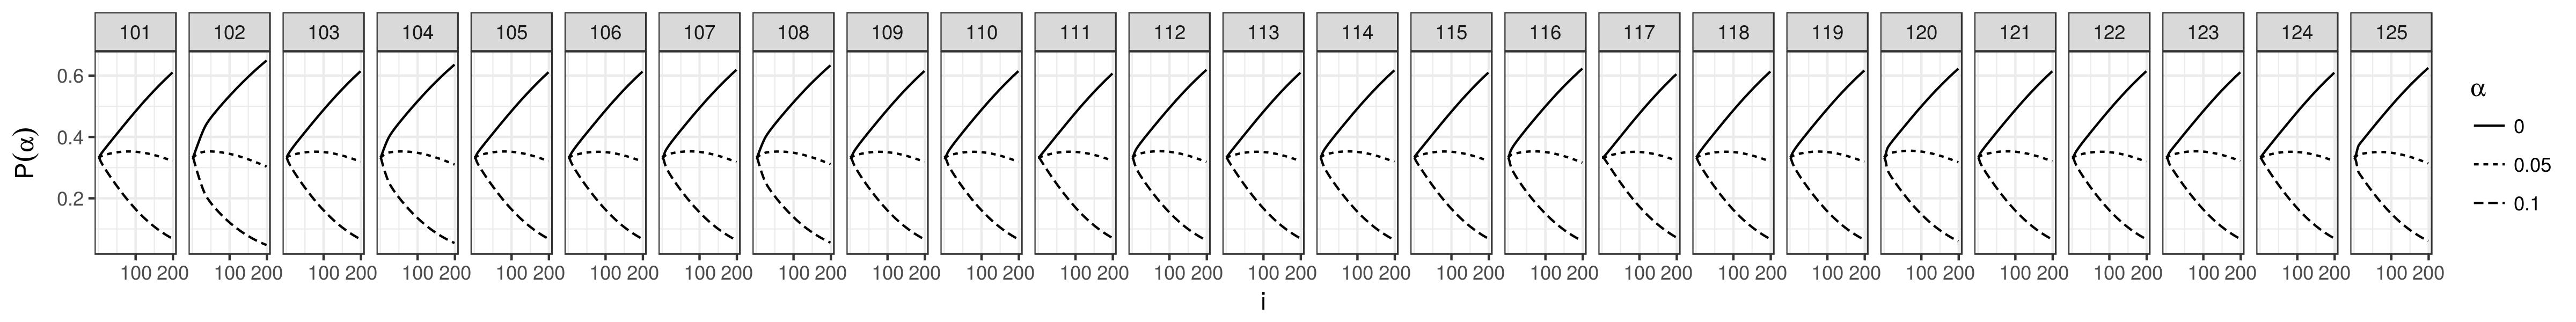
\includegraphics[width=\textwidth]{simulation/results/round-3/plots/proportion-cases-0-005-01-strong.png}
    \caption{Three populations scenario.}
    \label{fig:proportion-cases-three-tight-interaction}
  \end{subfigure}
  \caption{Evolution of population proportions through time for each simulation trial of the tight interaction model.}
  \label{fig:proportion-cases-tight-interaction}
\end{figure}
%\end{sidewaysfigure}
In Figure~\ref{fig:proportion-cases-tight-interaction} we plot the evolution of the proportion of each population in the two-population and three-populations scenario for all trials.
As the plot shows, for every trial, the population with no imprecision steadily increased its proportion against the others.
In the three population scenario, the proportion of type $\alpha = 0.05$ sees a slight increase in the beginning of the simulation, but inexorably starts a downward trend.
These observations go against the expectation of~\textcite{franke_vagueness_2017} that faster convergence to a convex strategy by populations with a certain level of imprecision could give them a temporary advantage to take over and eliminate other types.
The reason for this is interesting in itself.
What happens is that, because of the tight interaction between populations, the strategies of each type evolve in close tandem with each other.
One of the consequences of this is that the population with no imprecision reaches convexity faster than it would on its own because of the interaction with the populations with imprecision.
We can see this effect by looking into the percentage of trials with convex sender strategies at a given iteration, for each scenario, and comparing the three scenarios: population with no imprecision evolving alone, two populations ($\alpha \in \{0, 0.05\}$), and three populations ($\alpha \in \{0, 0.05, 0.1\}$).
\begin{figure}
  \centering
  \begin{subfigure}[]{0.32\textwidth}
    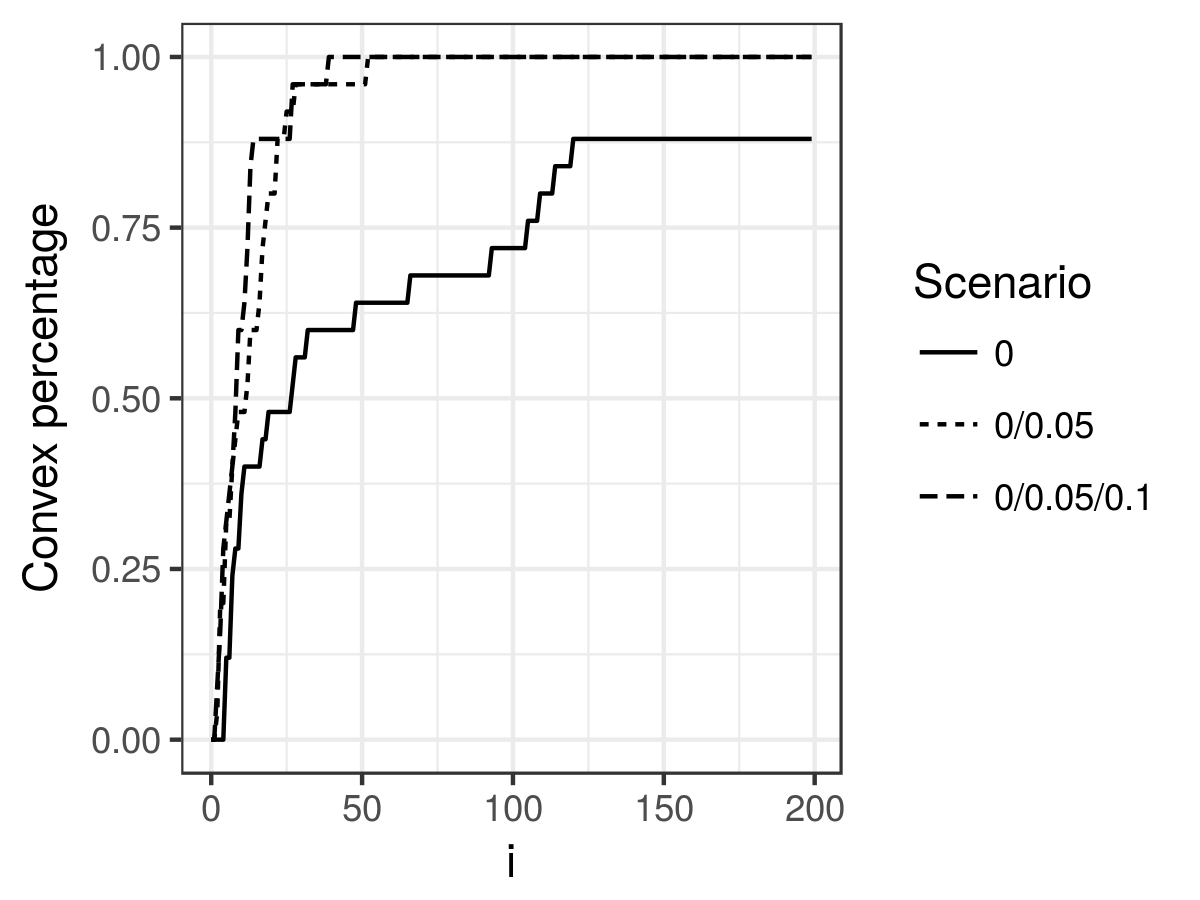
\includegraphics[width=\textwidth]{simulation/results/round-3/plots/convex-percentage-all-strong.png}
    \caption{Percentage of convex sender strategies for $\alpha = 0$.}
    \label{fig:convexity-tight-interaction}
  \end{subfigure}
  \hfill
  \begin{subfigure}[]{0.32\textwidth}
    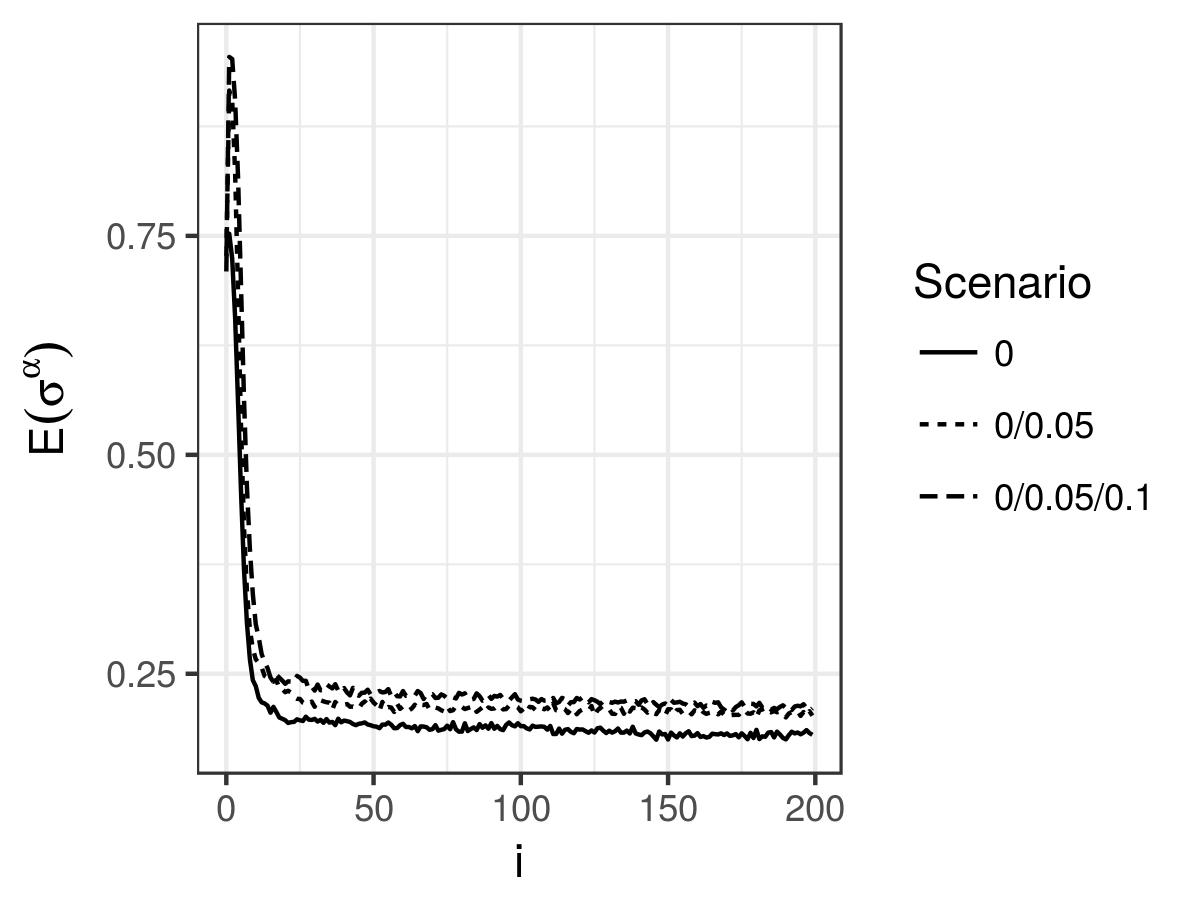
\includegraphics[width=\textwidth]{simulation/results/round-3/plots/entropy-sender-all-strong.png}
    \caption{Mean entropy of sender strategies for $\alpha = 0$.}
    \label{fig:entropy-sender-tight-interaction}
  \end{subfigure}
  \hfill
  \begin{subfigure}[]{0.32\textwidth}
    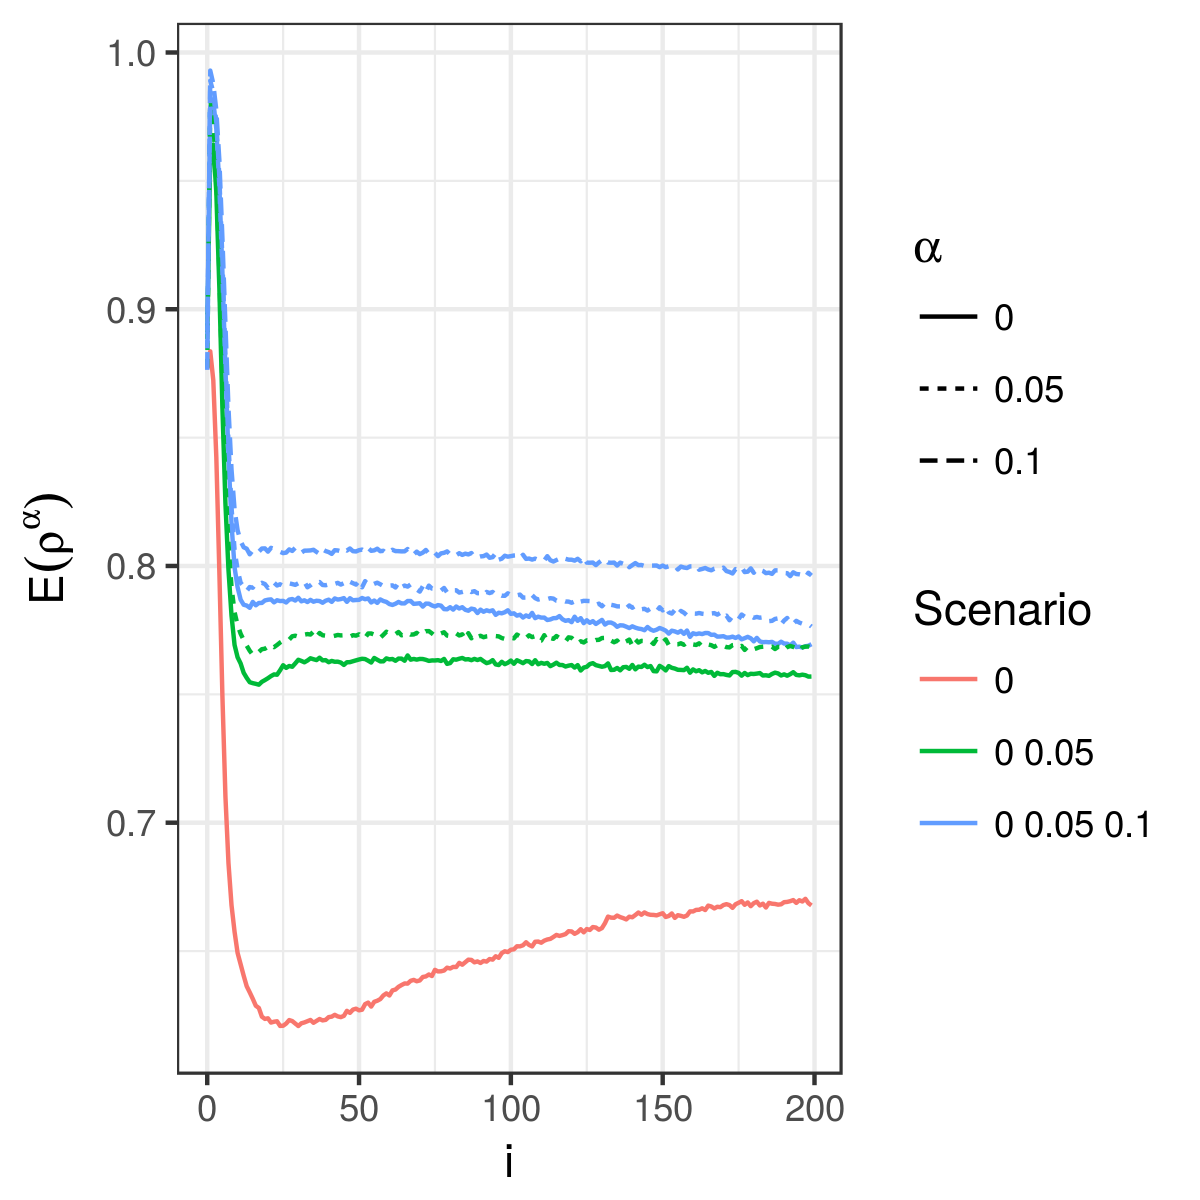
\includegraphics[width=\textwidth]{simulation/results/round-3/plots/entropy-receiver-all-strong.png}
    \caption{Mean entropy of receiver strategies for $\alpha = 0$.}
    \label{fig:entropy-receiver-tight-interaction}
  \end{subfigure}
  \caption{Development of some metrics through time for the $\alpha = 0$ population in each of three scenarios: evolving alone (`0'), with an $\alpha = 0.05$ population (`0/0.05'), and with an additional $\alpha = 0.1$ population (`0/0.05/0.1').}
  \label{fig:metrics-tight-interaction}
\end{figure}
This is plotted in Figure~\ref{fig:convexity-tight-interaction}.
What we see is more trials reaching convexity earlier for the multi-population scenarios when compared with the single-poulation scenario.
This effect precludes the hypothesized temporary advantage of imprecision to even manifest itself, but it can be seen as a positive influence on the population with no imprecision.

The flipside of this tight connection between populations is that strategies evolved by populations with no imprecision are also more vague (in the sense defined in Section~\ref{sec:sim-max-vagueness}).
This is visible by looking at mean entropy values, namely sender strategy entropy, plotted in Figure~\ref{fig:entropy-sender-tight-interaction}, and receiver strategy entropy, plotted in Figure~\ref{fig:entropy-receiver-tight-interaction}.
The values for the population with no imprecision are clearly higher in the scenarios where it evolves together with populations with imprecision than in the scenario where it evolves on its own.
Given the trends in population proportions, one expects this to eventually be eliminated when the population with no imprecision finally takes over the others, but it is interesting to observe that while populations with vague strategies persist, the population with no imprecision takes much longer to evolve a crisp strategy.


\subsection{Loose population interaction}
\label{sec:loose-interaction-model}
Given the tight interaction between populations precluding the manifestation of temporary advantages of vagueness, we decided to test a variation of the model where populations interact more loosely.
In order to do this, we need to make changes to some calculations.
However, any formula that is not redefined in this section should be assumed to remain the same.
The dynamic we want to model here is one where agents of a certain type $\alpha$ imitate and learn only from other agents of that same type.
First, if agents learn only within their population, the imitation dynamic needs to consider only the expected utility against agents of that population.
We thus define the following expected utilities for a sender of type $\alpha$:
$$
\text{EU}_{\sigma}^{\alpha}(m,t_{o},\rho^{\alpha})=\sum_{t_{a}}P_{\bar{o}}^{\alpha}(t_{a}|t_{o})\sum_{t_{r}}P_{\rho}^{\alpha}(t_{r}|m)U(t_{a},t_{r})
$$
and for a receiver of type $\alpha$:
$$
\text{EU}_{\rho}^{\alpha}(t_{i},m,\sigma^{\alpha})=\sum_{t_{a}}P_{\bar{\sigma}}^{\alpha}(t_{a}|m)\sum_{t_{r}}P_{r}^{\alpha}(t_{r}|t_{i})U(t_{a},t_{r})
$$
The main difference with the previous model is that these expected utilities are not calculated against all populations ($\sigma^\star$ and $\rho^\star$) but only against the agent's own type ($\sigma^\alpha$ and $\rho^\alpha$).
This also implies that population proportions do not play a role.

Regarding the imitation process, we can redefine the probability that a sender of type $\alpha$ observes a randomly sampled agent play message $m$ for observed state $t_o$ as:
$$
P_{o}^{\alpha}(m|t_{o})=\sum_{t_{a}}P_{\bar{o}}^{\alpha}(t_{a}|t_{o})P_{\sigma}^{\alpha}(m|t_{a})
$$
and the probability that a receiver of type $\alpha$ observes a randomly sampled agent choose interpretation $t_o$ given message $m$ as:
$$
P_{o}^{\alpha}(t_{o}|m)=\sum_{t_{r}}P_{o}^{\alpha}(t_{o}|t_{r})P_{\rho}^{\alpha}(t_{r}|m)
$$
Again, the main difference is that agents make observations within their own population, so to model a randomly sampled agent one needs only to take into account agents of the same type.
Population proportions again do not play a role in these calculations.
Based on these formulas, we can define the update probabilities for a sender strategy of type $\alpha$ at time instant $i+1$ as:
$$
\sigma_{i+1}^{\alpha}(m|t) \propto P_{o}^{\alpha}(m|t)\text{EU}_{\sigma_{i}}^{\alpha}(m,t,\rho_{i}^{\alpha})
$$
and similarly for a receiver strategy of type $\alpha$ as:
$$
\rho_{i+1}^{\alpha}(t|m) \propto P_{o}^{\alpha}(t|m)\text{EU}_{\rho_{i}}^{\alpha}(t,m,\sigma_{i}^{\alpha})
$$
Note that, because imitation and learning occur only within populations, these formulations are essentially the same as for the single-population model of~\textcite{franke_vagueness_2017}, only parameterized by type $\alpha$.

The selection process between different populations still follows the same motivation as before: agents of a certain type that evolve successful strategies (with respect to other types) will be more likely to survive and reproduce, benifiting the proportion of their population.
The formulation of the dynamic of the proportion of each type $P(\alpha)$ thus stays the same.
In order to avoid confusion, we want to stress that this means that these calculations rely on the definitions of expected utility across populations (\emph{i.e.}~$\text{EU}_{\sigma}^{\alpha}(m,t_{o},\rho^{\star})$ and $\text{EU}_{\rho}^{\alpha}(t_{i},m,\sigma^{\star})$) and not the newly introduced $\text{EU}_{\sigma}^{\alpha}(m,t_{o},\rho^{\alpha})$ and $\text{EU}_{\rho}^{\alpha}(t_{i},m,\sigma^{\alpha})$.

We ran the same number of simulation trials under the same conditions as for the model with tight population interaction.
%\begin{sidewaysfigure}
\begin{figure}
  \centering
  \begin{subfigure}[]{\textwidth}
    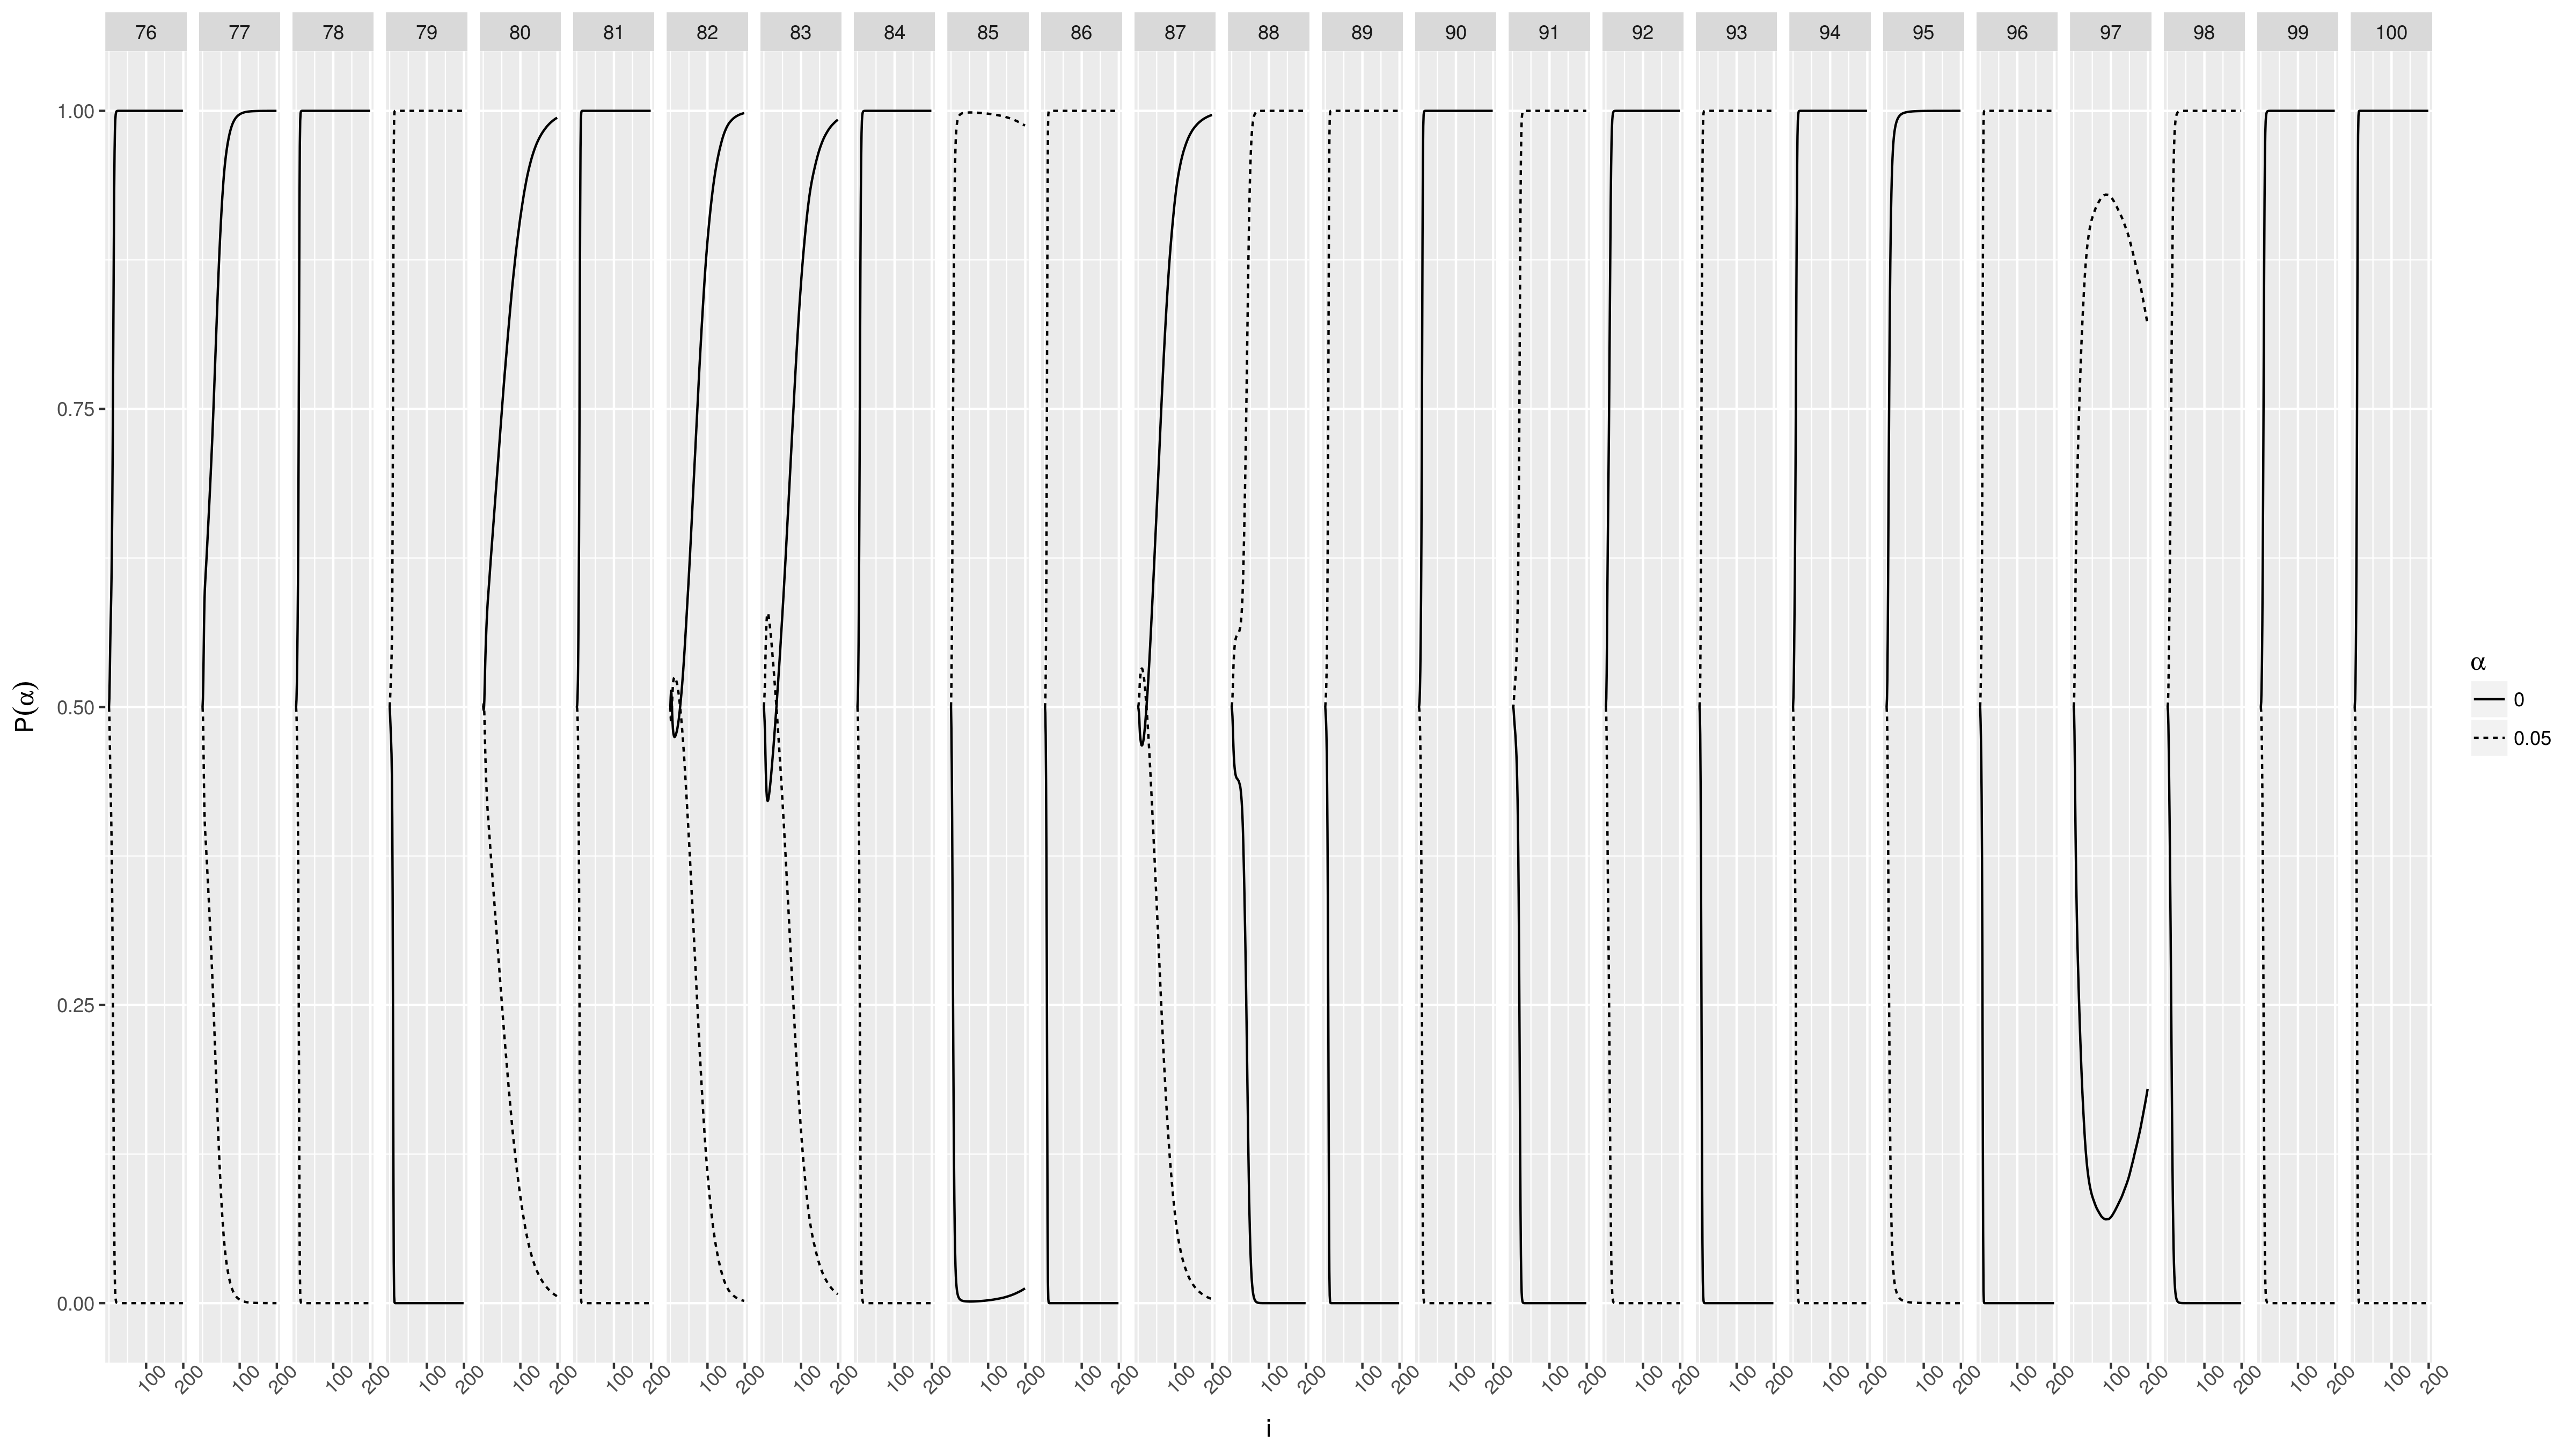
\includegraphics[width=\textwidth]{simulation/results/round-3/plots/proportion-cases-0-005-weakest.png}
    \caption{Two populations scenario.}
    \label{fig:proportion-cases-two-loose-interaction}
  \end{subfigure}
  \hfill
  \begin{subfigure}[]{\textwidth}
    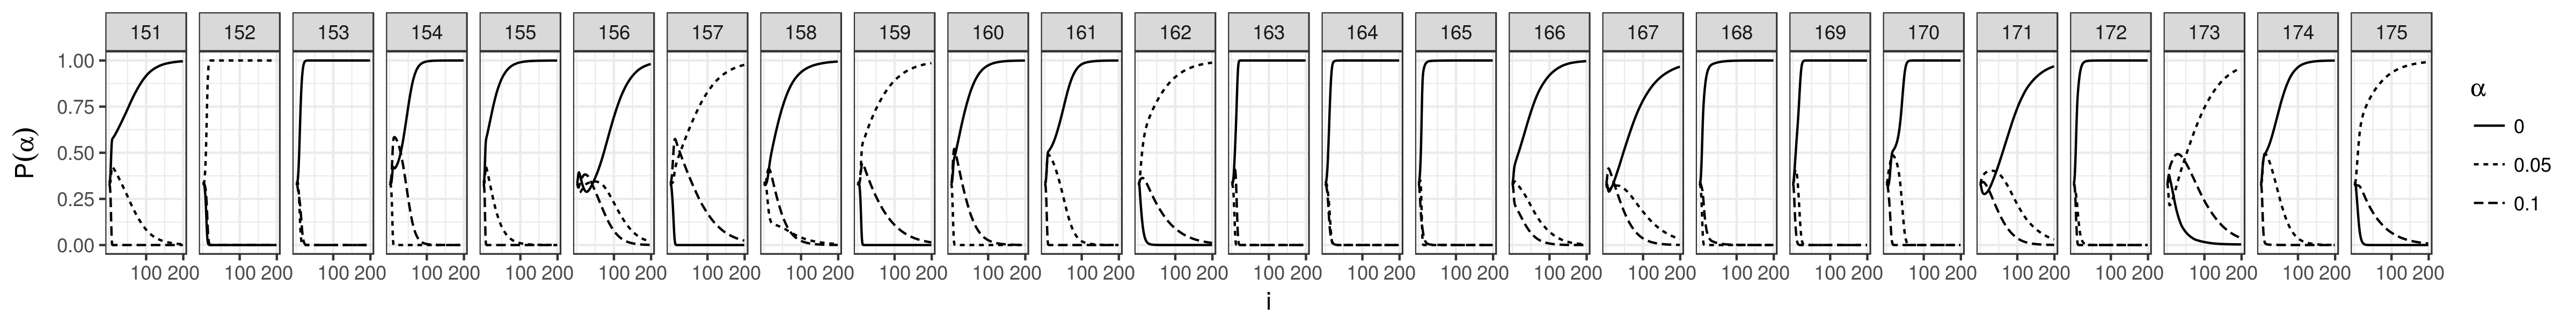
\includegraphics[width=\textwidth]{simulation/results/round-3/plots/proportion-cases-0-005-01-weakest.png}
    \caption{Three populations scenario.}
    \label{fig:proportion-cases-three-loose-interaction}
  \end{subfigure}
  \caption{Evolution of population proportions through time for each simulation trial of the loose interaction model.}
  \label{fig:proportion-cases-loose-interaction}
\end{figure}
%\end{sidewaysfigure}
In Figure~\ref{fig:proportion-cases-loose-interaction} we plot the evolution of population proportions for all trials of the multi-population scenarios.
The first thing to observe is that proportions evolve faster than in the model with tight interaction.
Whereas in the latter no given population ever reached much more than 70\% proportion, in this model we see that many trials resulted in one population fully dominating the others.
In the two-population scenario, some population reached 99\% proportion in 24 out of 25 trials.
In the three-population scenario, this happened in 18 out of 25 trials.
%Given that strategies no longer develop in close tandem with each other, differences in expected utility can become more salient resulting in some type reaching a more clear advantage than the other.
More interestingly for our investigation, some trials actually resulted in a population with some degree of imprecision dominating the others.
For the two-population scenario, $\alpha = 0.05$ fully reached 100\% proportion in 8 trials (79, 86, 88, 89, 91, 93, 96, 98), a point from which it is technically impossible for the other population to recover.
In most cases the dominating population gains its ground from the start, but in 5 cases we see a temporary advantage of $\alpha = 0.05$ that is then lost to the other population.
In one interesting trial (85), $\alpha = 0.05$ reached 99.87\% only to then steadly lose ground to $\alpha = 0$.
For the three population scenario, $\alpha = 0$ was reduced to 0\% proportion in 4 trials (152, 157, 159, and 175).
In all of those cases, $\alpha = 0.05$ clearly has the upper hand over $\alpha = 0.1$, despite a temporary advantage of the latter in some trials.
%In 5 other trials we see a positive trend for $\alpha = 0.05$, but given the reversals that sometimes occur (\emph{e.g.}~trial 171), one cannot be sure whether full dominance would be achieved if the simulation was left to run for longer time.

Because of the loose interaction between populations, different types can now evolve separately.
One consequence of this is that populations would a certain level of imprecision again reach convexity faster than those without imprecision.
\begin{figure}
  \centering
  \begin{subfigure}[]{0.45\textwidth}
    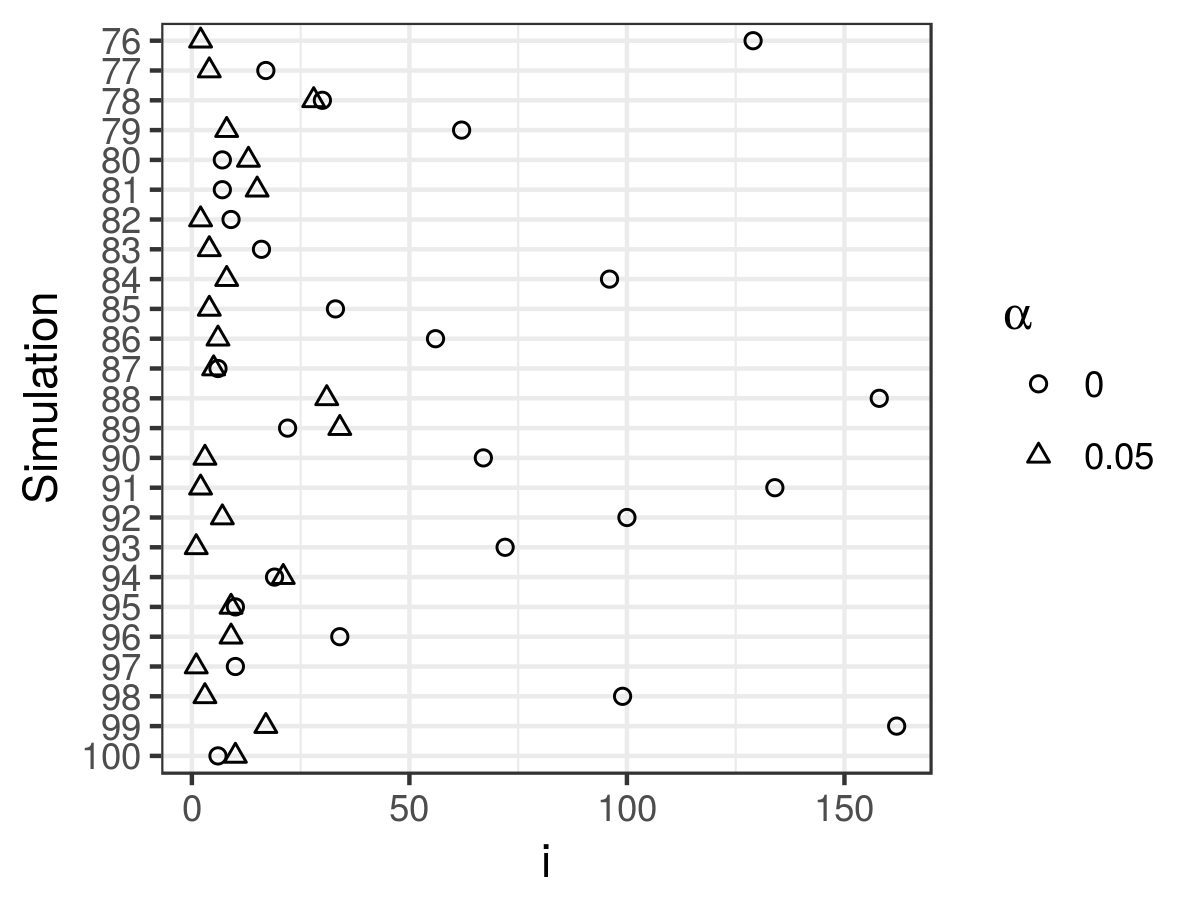
\includegraphics[width=\textwidth]{simulation/results/round-3/plots/convex-cases-0-005-weakest.png}
    \caption{Two populations scenario.}
    \label{fig:convex-cases-two-loose-interaction}
  \end{subfigure}
  \hfill
  \begin{subfigure}[]{0.45\textwidth}
    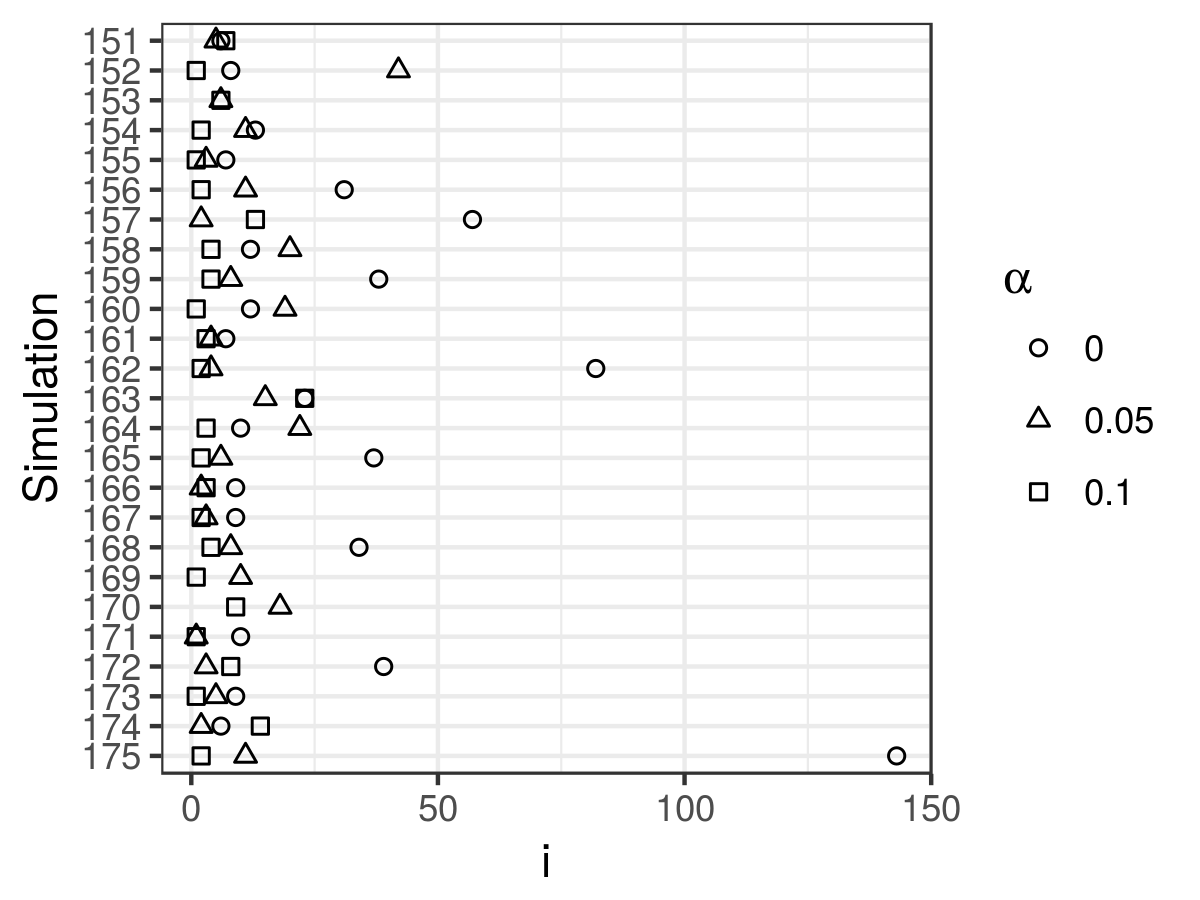
\includegraphics[width=\textwidth]{simulation/results/round-3/plots/convex-cases-0-005-01-weakest.png}
    \caption{Three populations scenario.}
    \label{fig:convex-cases-three-loose-interaction}
  \end{subfigure}
  \caption{First iteration with convex sender strategies for each simulation trial of the loose interaction model.}
  \label{fig:convex-cases-loose-interaction}
\end{figure}
In Figure~\ref{fig:convex-cases-loose-interaction} we plot, for each trial, the first iteration when each type reached convexity.
What we see is that, even though that is true on average, it is not always the case.
This has certainly to do with the initial conditions of each trial, since the randomly generated strategies can simply by chance be more favourable to reaching convexity.
More importantly, we also see that reaching convexity sooner is not a suficient condition for achieving population dominance .
There were many trials where another type reached convexity much sooner than $\alpha = 0$ but was completely dominated nevertheless (\emph{e.g.}~76, 84, 92, and 99 in the two-population scenario; 156, 165, 168, and 172 in the three-population scenario).
It also does not seem to be fully necessary, given a few examples where $\alpha = 0$ reached convexity early on and another type ended up dominating (89 in the two-population scenario and 152 in the three-population scenario).

Another consequence of the two populations evolving separately is that they do not necessarily evolve towards the same equilibrium.
In a sim-max game such as the one set up there are only two stable equilibria.
These are two Voronoi systems of the kind shown in Figure~\ref{fig:example_strats}, one where the first message is used for the first half of the state space, and the other where the second message is used for this region.
In the multi-population model with loose interaction, each population evolves independently towards one of these two equilibria.
This is importantly conditioned by the initial strategy the process of selection initiates from.
The populations are, however, not fully independent, since the process of selection of the level of precision relies on the expected utility of one population playing against itself and the others.
And this is important because strategies in one equilibrium get the lowest payoff possible against strategies in the other equilibrium.
Now, if two populations evolve towards different equilibria, whatever advantage one population has playing against itself could trigger a runaway effect by causing an increase in its proportion, which in turn will increase the population's relative expected utility, potentially increasing their proportion further in the next round, and so forth.
In this case, one would expect that faster convergence towards convexity would be especially important for success.

In the two-population scenario, of the 8 trials where $\alpha = 0$ was reduced to 0\%, all but two (88, 98) ended with the two populations each close to a different equilibria.
In the two-population scenario, the population with $\alpha = 0$ evolved towards the same equilibrium as the other two in 1 of the trials where it was eliminated.
In the other 3 trials, in 2 it evolved to a different equilibrium than the other two, and in 1 it evolved towards the same equilibrium as $\alpha = 0.05$ (but different to the one $\alpha = 0.1$ evolved towards).
Again, we do not find a clear case for this being a decisive factor in the success of populations with impairment.
That same goes for the impact of an initial advantage in expected utility creating the runaway effect we just mentioned.
Despite none of these three factors (including reaching convexity sooner) sentencing the demise of $\alpha = 0$ with certainty, they do seem to conspire together to bring it about.
In most trials where the type was eliminated, in both the two- and three-population scenarios, $\alpha = 0$ ended up evolving towards a different equilibrium than the other types, and either had an initial disadvantage in expected utility, or reached convexity much later.
These factors can thus be seen as indicators at best, but the story of how a population with imprecision ends up dominating one without seems to be more complicated to tell.

This is not surprising since we are facing a complex dynamical system with various interacting components (sender and receiver strategies and multiple populations).
\begin{figure}
  \centering
  \begin{subfigure}[]{0.45\textwidth}
    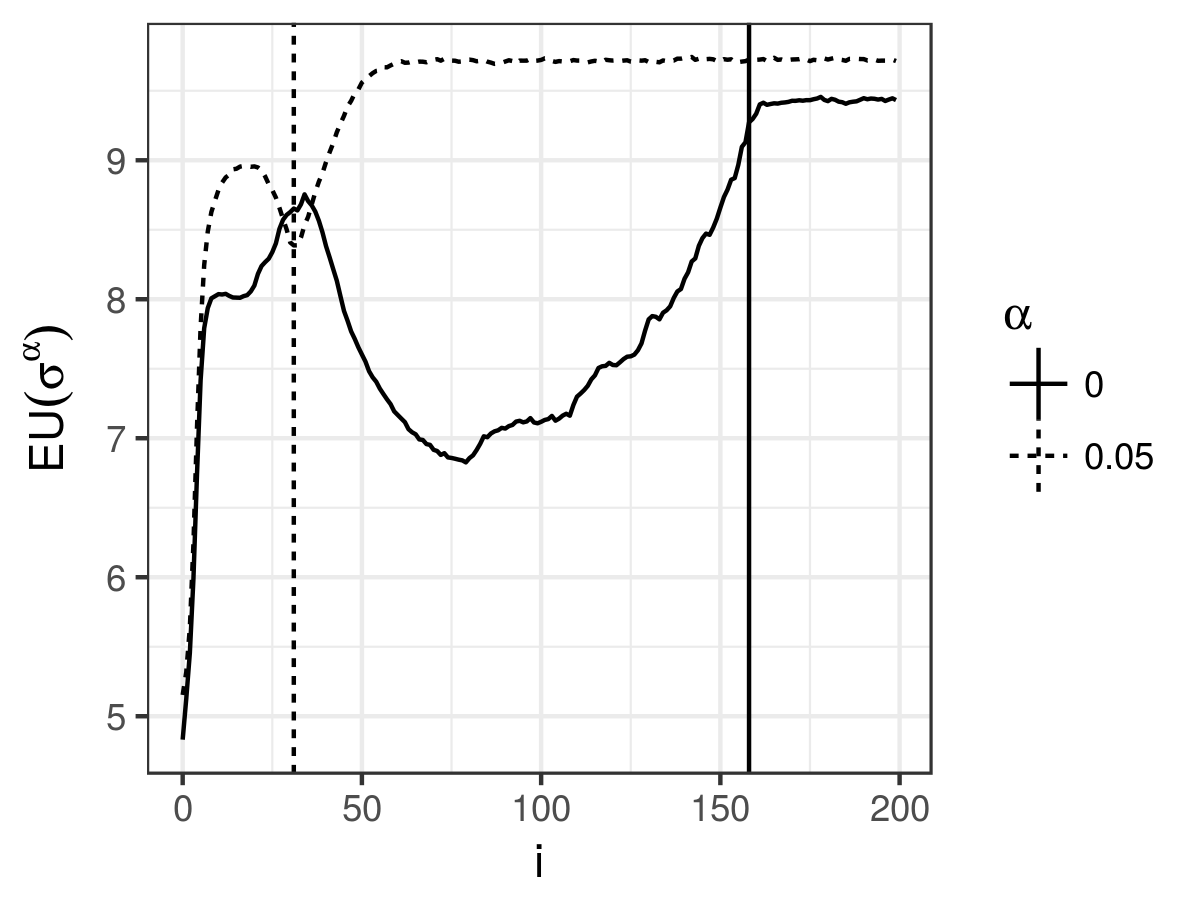
\includegraphics[width=\textwidth]{simulation/results/round-3/plots/sender-eu-trial-88-0-005-weakest.png}
    \caption{Sender expected utility.}
    \label{fig:sender-eu-trial-88-loose-interaction}
  \end{subfigure}
  \hfill
  \begin{subfigure}[]{0.45\textwidth}
    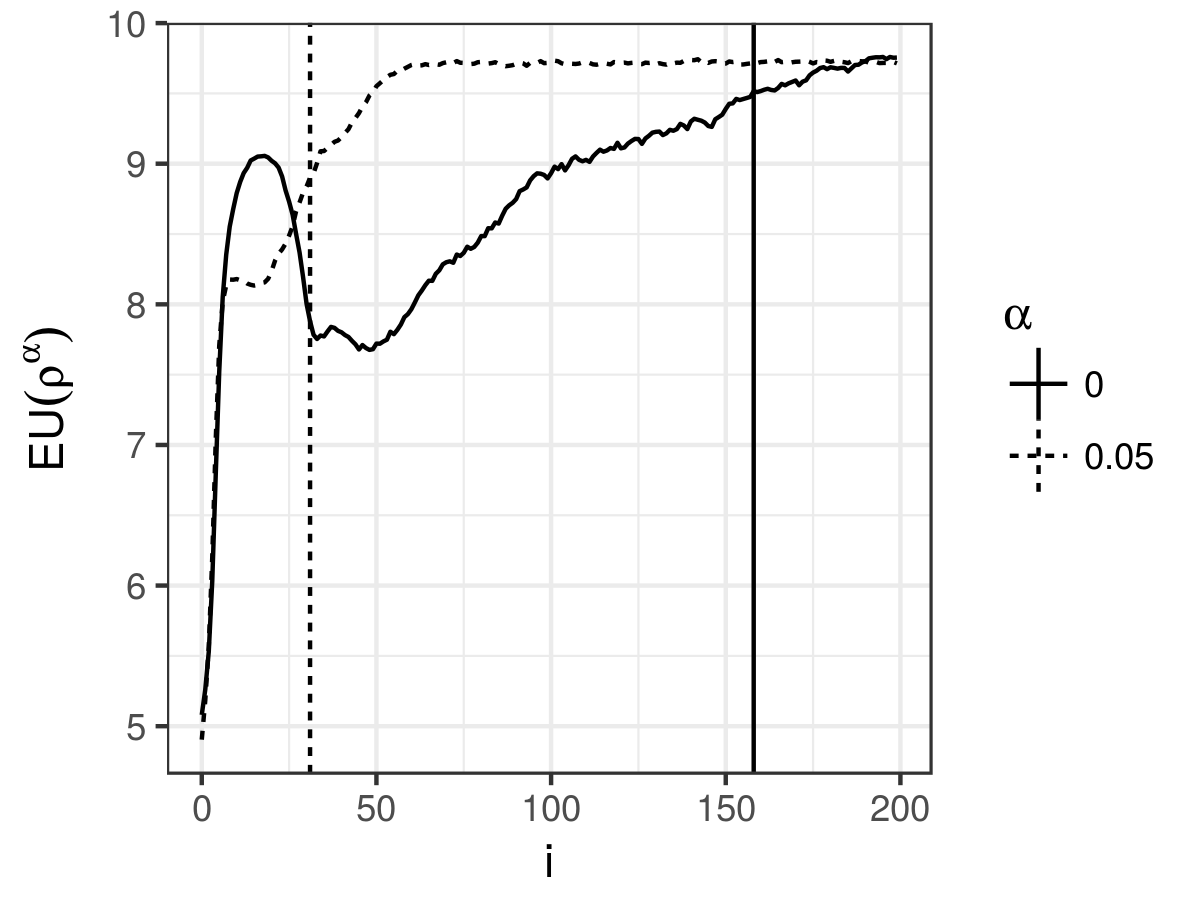
\includegraphics[width=\textwidth]{simulation/results/round-3/plots/receiver-eu-trial-88-0-005-weakest.png}
    \caption{Receiver expected utility.}
    \label{fig:receiver-eu-trial-88-loose-interaction}
  \end{subfigure}
  \caption{Expected utilities for trial 88 of the loose interaction model. Vertical lines demarcate, for each type, the iteration where convexity was achieved.}
  \label{fig:eu-trial-88-loose-interaction}
\end{figure}
Just as an example of this, in Figure~\ref{fig:eu-trial-88-loose-interaction} we plot the expected utilities of sender and receiver strategies for both populations of trial 88.
The curves up to where $\alpha = 0.05$ achieved convexity seem to suggest that the sender strategy of that type was evolving in tandem with the receiver strategy of the other.
This is possible in our model, although we expect it to be highly unlikely.
The moment where the population reaches convexity marks the point where the sender strategy of $\alpha = 0.05$ aligns with its type's receiver strategy and this coincides with the moment where the population seems to gain real traction over the other type (see again the plot for trial 88 in Figure~\ref{fig:convex-cases-loose-interaction}).


\section{Conclusions}
\label{sec:conclusions}
\todo[inline]{Extend/Rewrite}
We tried to show that, if we pragmatically acknowledge the complex and dynamic environment that surrounds language learning and use, we find many plausible sources of uncertainty that can lead to vague signal use.
We supported this claim by giving an overview of recent research that tries to accommodate for vagueness in the context of sim-max games, and by discussing, in more general terms, how these considerations are relevant for reference games, and in the broader context of language as a multiplicity of language-games.
Furthermore, we argued that if we broaden our notion of rationality beyond mere maximization of expected utility, we also find reasons to welcome the positive aspects of these processes and to see their acceptance as a perfectly rational choice.
Irrational would be to ignore the finite nature of our existence and the constraints that condition language learning and use.
Our challenge as researchers is of course not only to draw attention to the possibilities, but also to characterize which particular constraints give rise to vague signal use and how.

The investigation doesn't end here, then.
The research discussed here suggests that although vagueness can be beneficial, that is the case only in moderation: too much can lead to babbling equilibria where no information is transmitted.
Thus, for agents capable of adjusting the level of vagueness in their strategies, questions remain regarding how this can be modeled and what factors influence the amount of vagueness that is optimal for a given situation.
Other challenges include how to incorporate into our models the intuitions about the importance of speed of convergence, adaptability, and the promotion of group homogeneity.
Finally, perhaps the biggest of them all is how to be able to focus on one language-game without losing sight of the ecosystem of games that need to be taken into account as well.
Whatever solutions we find to these challenges, we believe that a notion of rationality cannot be strongly tied to mere utility maximization in a particular game, but has to consider an agents' need to optimize his behavior to navigate the plurality of uncertainties that besiege him.
We need a clear notion of ecological rationality in order to see vagueness in the right light.


\printbibliography

\end{document}
